\documentclass[unicode,10pt,a4paper,oneside,numbers=endperiod,openany]{scrartcl}
\usepackage[backend=biber,style=numeric]{biblatex}
\addbibresource{references.bib}
\usepackage{tikz}
\usepackage{pgfplots}
\usepgfplotslibrary{colorbrewer} % better colors
\pgfplotsset{compat=1.18}
\usepackage{amsmath}
\usepackage{url}
\usepackage{xcolor}
\usepackage{subcaption}
\usepackage{listings}
\usepackage{multirow}
\usepackage{graphicx}
\lstdefinestyle{grayverbatim}{
  basicstyle=\ttfamily,%
  backgroundcolor=\color{gray!10},%
  frame=single,%
  framesep=3pt,%
  breaklines=true,%
  columns=fullflexible%
  numberstyle = \tiny,%
  stepnumber = 1,%
  numbersep = 5pt,%
  numbers = left%
}
\definecolor{lightbluehighlight}{RGB}{204,232,255}
\input{assignment.sty}

\begin{document}


\setassignment
\setduedate{\textbf{Friday} 22 May 2026, 18:00~(Europe/Zurich)}

\serieheader{High-Performance Computing Lab for CSE}{2026}
            {Student: Riccardo Polo}
            {Discussed with: Giovanni Guidarini}
            {Solution for Project 6}{}
\newline

\assignmentpolicy

\newpage

\section{Graph Partitioning with Julia: Load balancing for HPC [50 points]}
\subsection{Graph Partitioning Algorithms}
\subsubsection{Inertial Bisection algorithm}

Listing~\ref{lst:inertial_bisection} reports the implementation of the inertial bisection algorithm. 
This method uses the geometrical information associated with the graph vertices, namely their
coordinates, to split the graph into two subdomains. The basic idea is to interpret the vertices as a
set of points in the plane and to compute the direction along which the point cloud has the largest
spatial spread. The graph is then partitioned by projecting the vertices onto this direction and
separating them according to their position with respect to a cutting line.

\begin{lstlisting}[style=grayverbatim, caption={Inertial Bisection algorithm}, label={lst:inertial_bisection}]
function inertial_part(A, coords)

    p = ones(Int, size(coords, 1))

    xbar = mean(coords[:, 1])
    ybar = mean(coords[:, 2])

    Sxx = sum((coords[:, 1] .- xbar) .^ 2)
    Syy = sum((coords[:, 2] .- ybar) .^ 2)
    Sxy = sum((coords[:, 1] .- xbar) .* (coords[:, 2] .- ybar))

    M = Symmetric([Syy -Sxy;
                   -Sxy Sxx])

    eigvals, eigvecs = eigs(M; nev=1, which=:SM)
    eigv = real.(eigvecs[:, 1])

    p1, p2 = partition(coords, eigv)

    p[p1] .= 1
    p[p2] .= 2

    return p
end
\end{lstlisting}
The function first initializes the partition vector \texttt{p}, assigning all vertices to the same
subdomain. The number of entries of \texttt{p} is equal to the number of rows of \texttt{coords}, hence to the number of vertices of the graph. \\
The quantities \texttt{xbar} and \texttt{ybar} represent the coordinates of the center of mass of the vertices. The coordinates are then shifted with respect to this center of mass in order to compute the second-order moments \texttt{Sxx}, \texttt{Syy}, and \texttt{Sxy}. These quantities measure the spatial distribution of the vertices around the center of mass: \texttt{Sxx} and \texttt{Syy} quantify the spread along the coordinate directions, while \texttt{Sxy} measures the correlation between the two coordinates.\\

Using these moments, the matrix
\[
M =
\begin{pmatrix}
S_{yy} & -S_{xy} \\
-S_{xy} & S_{xx}
\end{pmatrix}
\]
is assembled as a symmetric matrix. The eigenvector associated with the smallest eigenvalue of
\texttt{M} defines the principal inertial direction of the point set. In the implementation, this
eigenvector is computed by calling \texttt{eigs} with \texttt{nev=1} and \texttt{which=:SM}, which selects the
eigenpair of smallest magnitude. Since the matrix is real and symmetric, the resulting eigenvector
is converted to its real part and stored in \texttt{eigv}.\\
The actual split is then performed by the auxiliary routine \texttt{partition(coords, eigv)}. This
routine projects the vertex coordinates onto the inertial direction and separates the vertices into
two sets, denoted by \texttt{p1} and \texttt{p2}. These two sets correspond to the two sides of the
bisecting line. Finally, the partition vector is updated by assigning label \texttt{1} to all vertices in \texttt{p1} and label \texttt{2} to all vertices in \texttt{p2}. The returned vector \texttt{p} therefore contains the bisection of the graph induced by the inertial direction.

\subsubsection{Spectral Bisection Algorithm}

In Listing~\ref{lst:spectral_bisection}, we report the implementation of the spectral bisection algorithm.
Unlike inertial bisection, this method does not use the geometrical coordinates of the vertices. Instead,
it exploits the connectivity structure of the graph through the graph Laplacian matrix. The main idea is
to compute an eigenvector of the Laplacian, known as the Fiedler vector, and use its components to divide
the vertices into two groups.

\begin{lstlisting}[style=grayverbatim, caption={Spectral Bisection algorithm}, label={lst:spectral_bisection}]
function spectral_part(A)

    n = size(A, 1)

    if n == 1
        return ones(Int, 1)
    end

    # 1. Construct the Laplacian matrix.
    D = Diagonal(vec(sum(A, dims=2)))
    L = Symmetric(Matrix(D - A))

    # 2. Compute eigendecomposition.
    eig = eigen(L)

    # 3. Take eigenvector associated with second smallest eigenvalue.
    perm = sortperm(eig.values)
    fiedler_vec = eig.vectors[:, perm[2]]

    # 4. Balanced partition by sorting the Fiedler vector.
    order = sortperm(fiedler_vec)

    p = ones(Int, n)

    n1 = div(n, 2)
    p[order[1:n1]] .= 1
    p[order[n1+1:end]] .= 2

    return p

end
\end{lstlisting}
The function takes as input the adjacency matrix \texttt{A} of the graph and first extracts the number
of vertices \texttt{n}. A special case is included for graphs with a single vertex: in this situation no
meaningful bisection can be performed, and the function simply returns a partition vector containing
one label.\\

The first step of the algorithm consists in constructing the graph Laplacian. The diagonal matrix
\texttt{D} contains the degrees of the vertices, computed by summing the rows of the adjacency matrix.
The Laplacian is then assembled as
\[
L = D - A.
\]
In the implementation, the matrix is explicitly converted to a symmetric matrix using
\texttt{Symmetric(Matrix(D - A))}. This is consistent with the fact that, for an undirected graph, the
Laplian is real and symmetric.\\
The spectral information of the graph is then obtained by computing the eigendecomposition of
\texttt{L}. The eigenvalues are sorted in increasing order, and the eigenvector associated with the
second smallest eigenvalue is selected. This vector is the Fiedler vector. The smallest eigenvalue of
the Laplacian is associated with the constant eigenvector and does not provide a useful separation of
the graph. The second smallest eigenvector, instead, contains information about the weakest connected
direction of the graph and is therefore used to define the bisection.\\

In the theoretical version of spectral bisection, the split can be obtained by comparing the components
of the Fiedler vector with a threshold, often chosen as zero or as the median value. In this implementation,
a balanced partition is enforced explicitly. The entries of the Fiedler vector are sorted, and the first
\texttt{div(n, 2)} vertices in this ordering are assigned to the first subdomain, while the remaining
vertices are assigned to the second subdomain. This guarantees that the two parts have approximately
the same number of vertices, which is desirable in recursive graph partitioning because it avoids strongly
unbalanced subdomains.\\

Finally, the partition vector \texttt{p} is returned. Its entries contain the labels of the two subdomains:
vertices assigned label \texttt{1} belong to the first part, while vertices assigned label \texttt{2} belong to
the second part.

\subsubsection{Results}
The script \texttt{main\_bench.jl} was used to run the four bisection strategies on the toy
meshes loaded by \texttt{bench\_bisection.jl}. For each mesh and each partitioning strategy, we
measured the bisection edge-cut, i.e. the number of graph edges whose endpoints belong to
different parts. Since the partitions are constrained to be balanced, the edge-cut provides a
simple measure of the quality of the interface between the two subdomains: lower values
correspond to fewer inter-partition connections and therefore to less communication in a
parallel graph-distributed computation.

\begin{table}[h]
\centering
\begin{tabular}{lcccc}
\hline
\textbf{Mesh} & \textbf{Coordinate} & \textbf{Inertial} & \textbf{Spectral} & \textbf{METIS} \\
\hline
\texttt{3elt}          & -- & -- & -- & -- \\
\texttt{airfoil1}      & -- & -- & -- & -- \\
\texttt{barth4}        & -- & -- & -- & -- \\
\texttt{crack}         & -- & -- & -- & -- \\
\texttt{mesh1e1}       & -- & -- & -- & -- \\
\texttt{mesh2e1}       & -- & -- & -- & -- \\
\texttt{mesh3e1}       & -- & -- & -- & -- \\
\texttt{netz4504\_dual} & -- & -- & -- & -- \\
\texttt{stufe}         & -- & -- & -- & -- \\
\texttt{ukerbe1}       & -- & -- & -- & -- \\
\hline
\end{tabular}
\caption{Bisection edge-cut obtained on the toy meshes loaded by \texttt{bench\_bisection.jl}.}
\label{tab:bisection_edgecuts}
\end{table}

The corresponding partitions are shown in Figures~\ref{fig:3elt_bisections}--\ref{fig:crack_bisections} for the first four meshes, in Figures~\ref{fig:mesh1e1_bisections}--\ref{fig:stufe_bisections} for the additional structured meshes, and in Figure~\ref{fig:ukerbe1_bisections} for the \texttt{ukerbe1} mesh.
The coordinate and inertial methods are purely geometrical: they only use the position of the
vertices and therefore tend to produce almost straight cuts. This behaviour is clearly visible in
the \texttt{3elt}, \texttt{barth4}, and \texttt{crack} examples. Such partitions are simple and often
reasonable when the mesh is approximately uniform and the graph connectivity follows the
geometry closely. However, they can become sub-optimal when the mesh has non-uniform density
or when the geometry contains local features that should not be cut through.\\

The spectral and METIS partitions are instead based on the graph connectivity. As a consequence,
they are generally more flexible: the interface is not restricted to be a straight geometrical line,
but can follow weaker connections in the graph. This is particularly important for meshes such as
\texttt{airfoil1}, where the local refinement around the airfoil and its wake makes a purely
geometrical split less adapted to the graph structure. In this case, the coordinate and inertial
cuts separate the mesh in a rather direct left-right fashion, while spectral bisection and METIS
produce more irregular interfaces that better reflect the connectivity of the mesh.\\

Some surprising or clearly sub-optimal partitions can also be observed. In particular, for
\texttt{barth4} the METIS and spectral results appear very unbalanced visually, with one part
concentrated around only a small region near the centre of the mesh. A similar behaviour appears
for the \texttt{3elt} mesh in the METIS and spectral plots, where one color occupies almost the
entire mesh and the other is concentrated in a very small central region. This suggests that either
the partition labels are not being displayed as expected, or that the returned partition is not a
proper balanced bisection for these cases. Since recursive bisection relies on each split producing
two meaningful subdomains, such cases should be checked carefully by verifying the number of
vertices assigned to each part in addition to the edge-cut value.\\

The additional structured meshes further illustrate the difference between geometrical and
connectivity-based partitioning. For the regular meshes \texttt{mesh1e1}, \texttt{mesh2e1}, and
\texttt{mesh3e1}, all methods produce relatively clean partitions, but the shape of the interface
depends on the criterion used by the algorithm. Coordinate bisection typically produces a vertical
or horizontal cut aligned with the coordinate axes, while inertial bisection may rotate the cut
according to the dominant spatial direction of the mesh. Spectral bisection and METIS may instead
introduce slightly irregular interfaces when this reduces the number of cut edges.\\

The \texttt{netz4504\_dual} and \texttt{stufe} meshes are more interesting because their geometry is
less uniform. In these cases, a purely geometrical cut does not necessarily correspond to the
smallest communication interface. The graph-based methods are able to adapt the separator to
the local connectivity of the mesh, especially around refined or stepped regions. This is the
expected behaviour: the objective of graph partitioning is not to produce a visually straight cut,
but to minimize the number of edges crossing between different parts while keeping the load
balanced.\\

Finally, the \texttt{ukerbe1} mesh shows a geometry with a pronounced notch-like feature and
several internal circular holes. In this case, the coordinate and inertial methods still produce
mostly straight cuts, separating the mesh approximately into upper and lower parts. This is
reasonable from the point of view of the global geometry, but it does not explicitly account for
the connectivity around the notch and the locally refined region. The spectral and METIS
partitions instead place the separator very close to this narrow central region. This behaviour is
consistent with the graph-based objective, since cutting through a geometrical bottleneck can
reduce the number of edges crossing between the two parts. However, the METIS partition appears
visually suspicious, since one part is concentrated in a very small region close to the notch while
the rest of the mesh belongs to the other part. As for the previous anomalous cases, this should be
checked against the actual part sizes printed by the script, because a low edge-cut is meaningful
only if the balance constraint is also satisfied.\\

Overall, the results confirm the expected trade-off between geometrical and graph-based
partitioning. Coordinate and inertial bisection are cheap and produce simple cuts, but they may
ignore important connectivity features. Spectral bisection and METIS can produce lower edge-cuts
because they exploit the graph structure directly, but the resulting partitions may be less regular
geometrically and, in some cases, should be inspected to ensure that the balance constraint has
been respected.

\begin{figure}[h]
\centering
\begin{subfigure}[b]{0.24\textwidth}
    \centering
    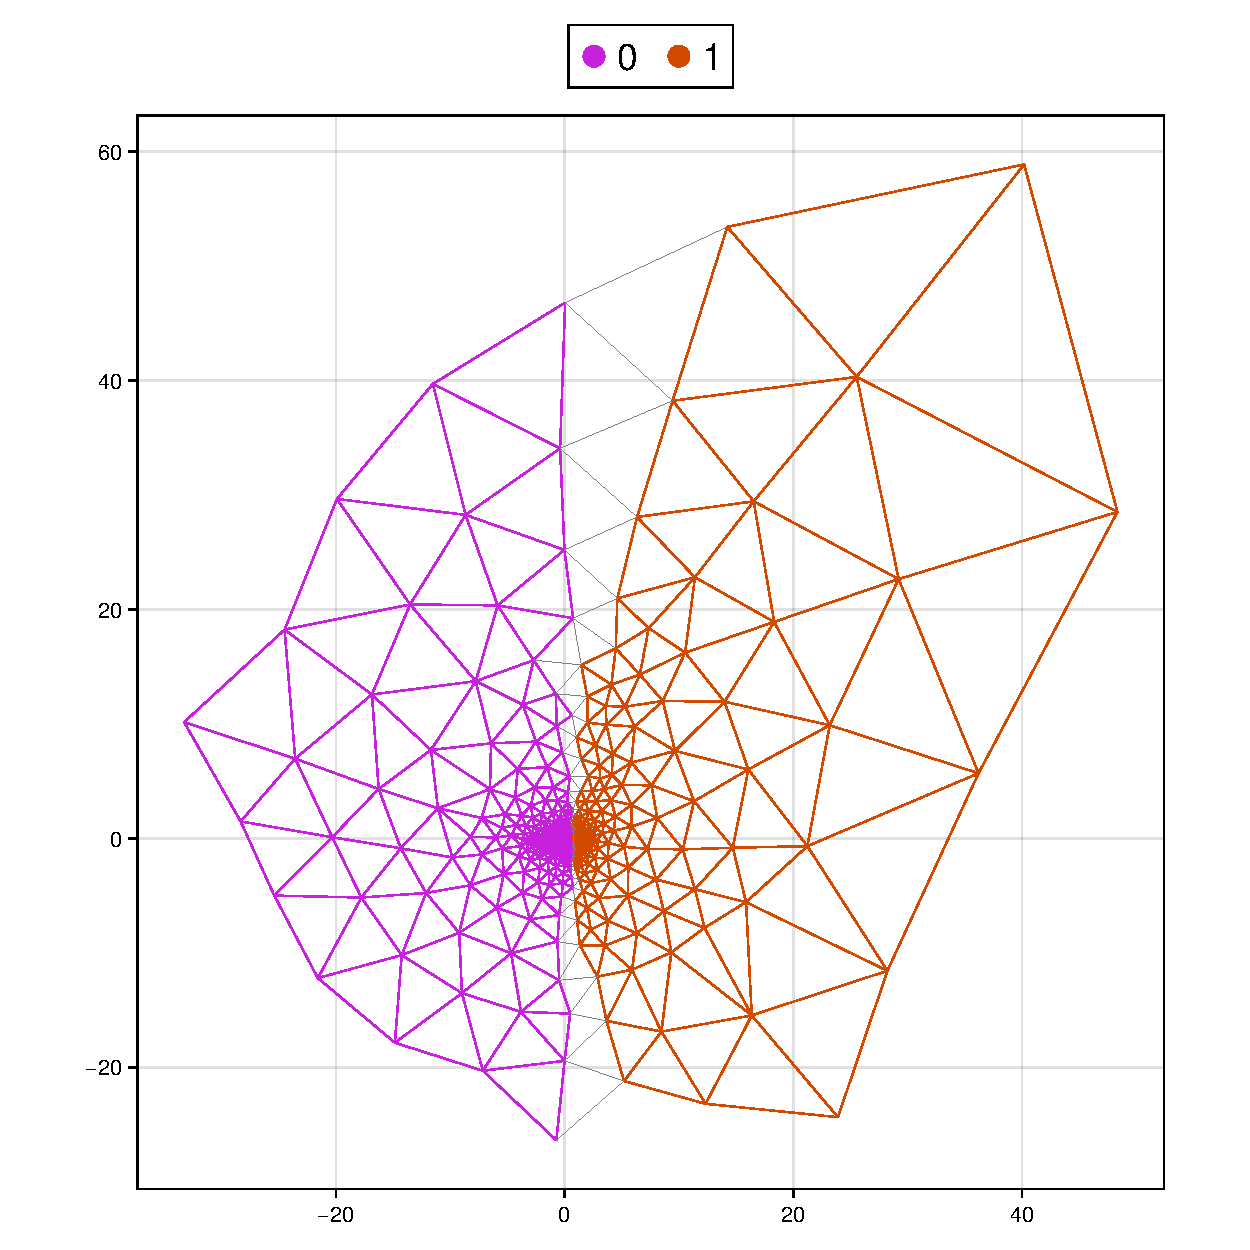
\includegraphics[width=\textwidth]{../01_graph/images/bisection/3elt_coordinate_bisection.pdf}
    \caption{Coordinate}
\end{subfigure}
\begin{subfigure}[b]{0.24\textwidth}
    \centering
    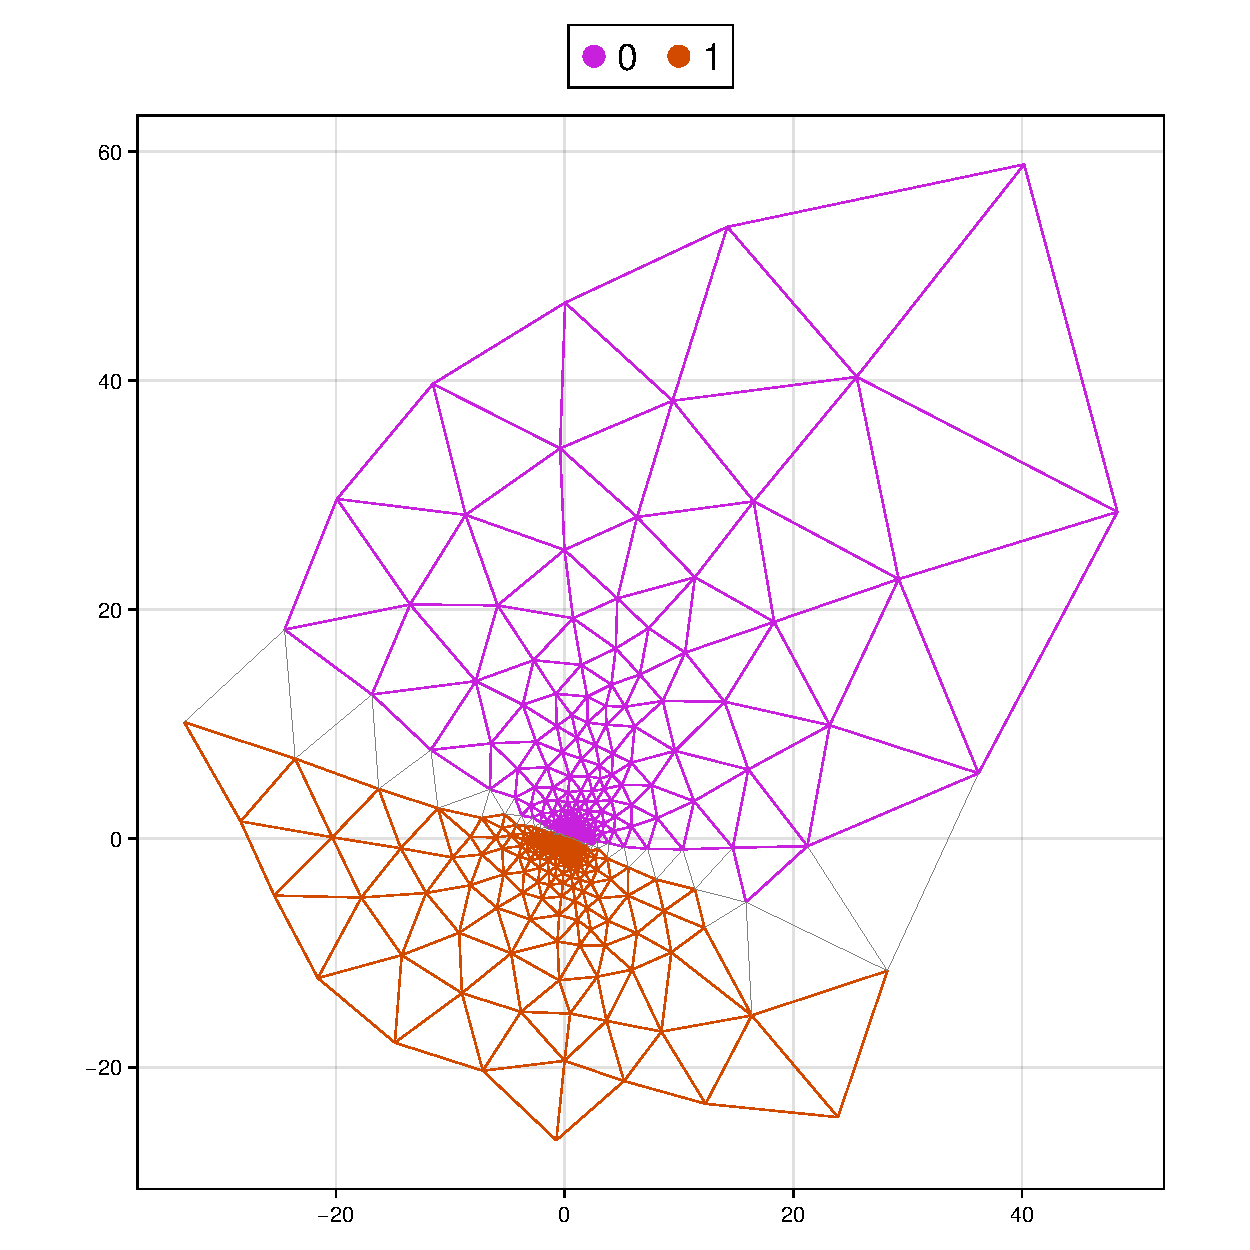
\includegraphics[width=\textwidth]{../01_graph/images/bisection/3elt_inertial_bisection.pdf}
    \caption{Inertial}
\end{subfigure}
\begin{subfigure}[b]{0.24\textwidth}
    \centering
    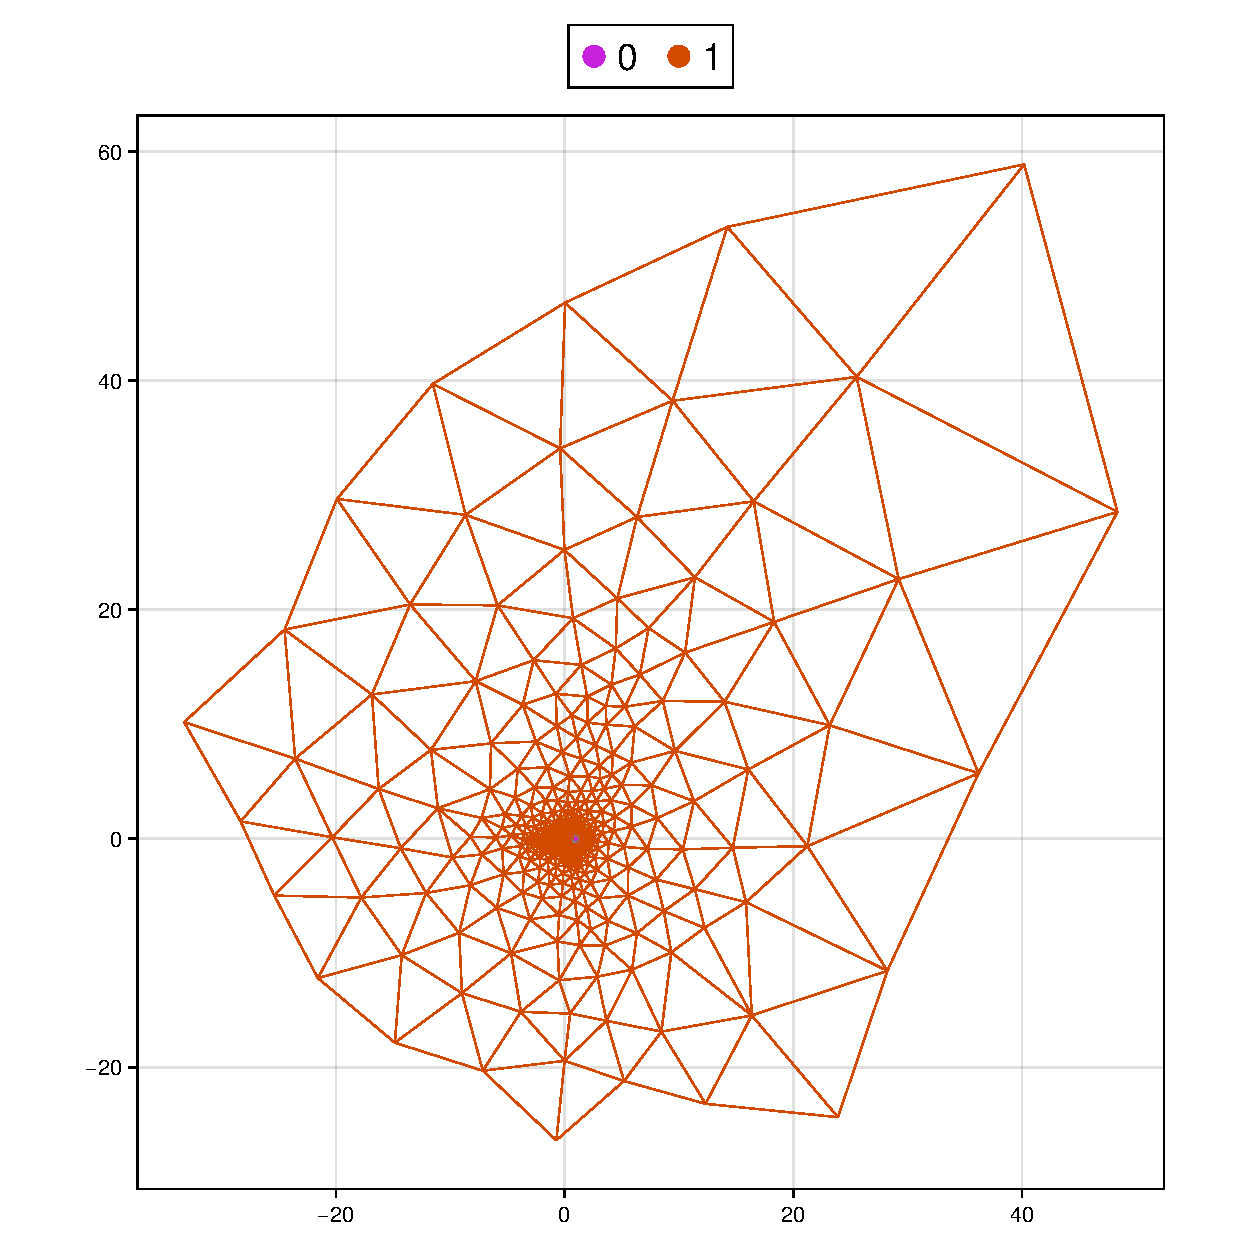
\includegraphics[width=\textwidth]{../01_graph/images/bisection/3elt_spectral_bisection.pdf}
    \caption{Spectral}
\end{subfigure}
\begin{subfigure}[b]{0.24\textwidth}
    \centering
    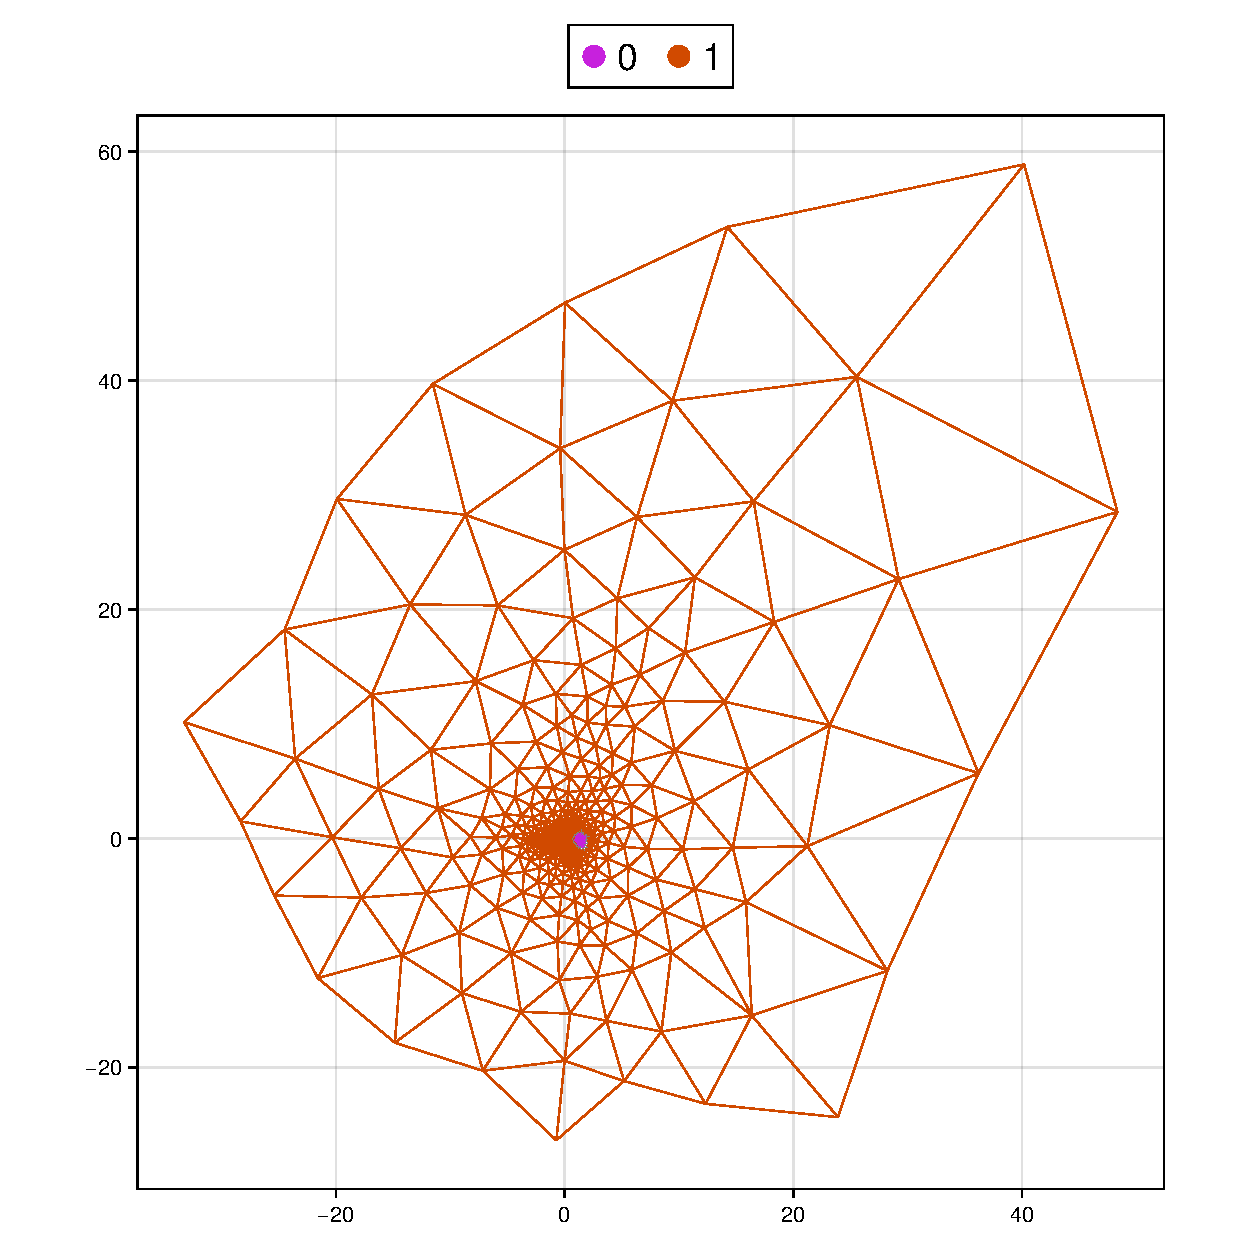
\includegraphics[width=\textwidth]{../01_graph/images/bisection/3elt_metis_bisection.pdf}
    \caption{METIS}
\end{subfigure}
\caption{Bisection partitions obtained for the \texttt{3elt} mesh.}
\label{fig:3elt_bisections}
\end{figure}

\begin{figure}[h]
\centering
\begin{subfigure}[b]{0.24\textwidth}
    \centering
    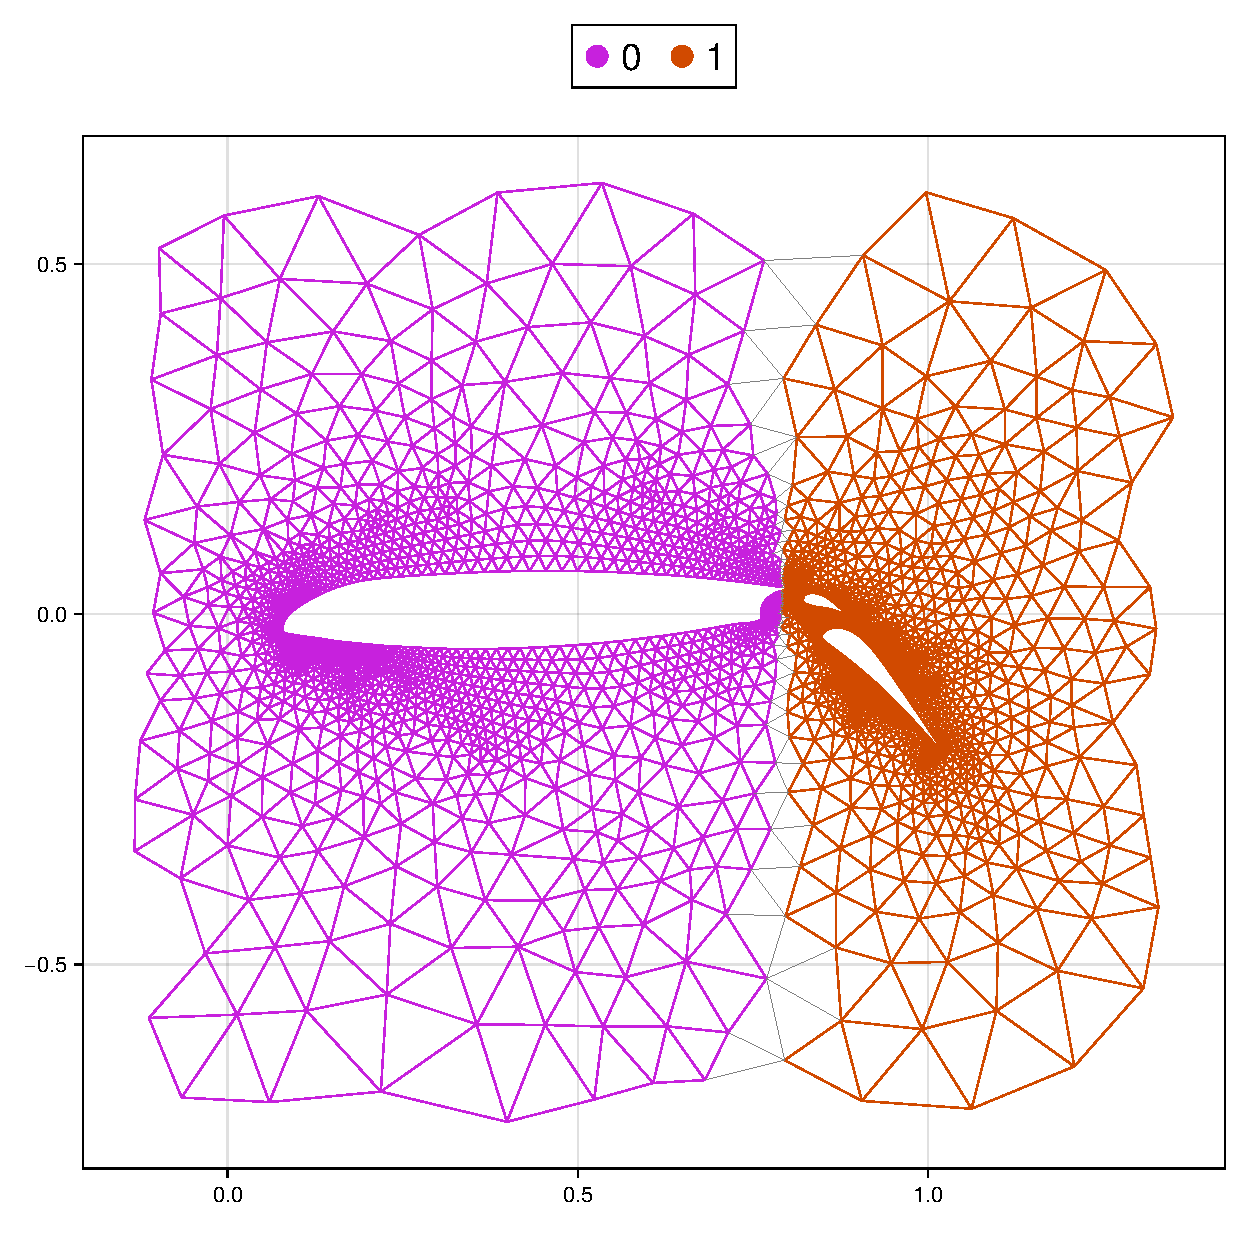
\includegraphics[width=\textwidth]{../01_graph/images/bisection/airfoil1_coordinate_bisection.pdf}
    \caption{Coordinate}
\end{subfigure}
\begin{subfigure}[b]{0.24\textwidth}
    \centering
    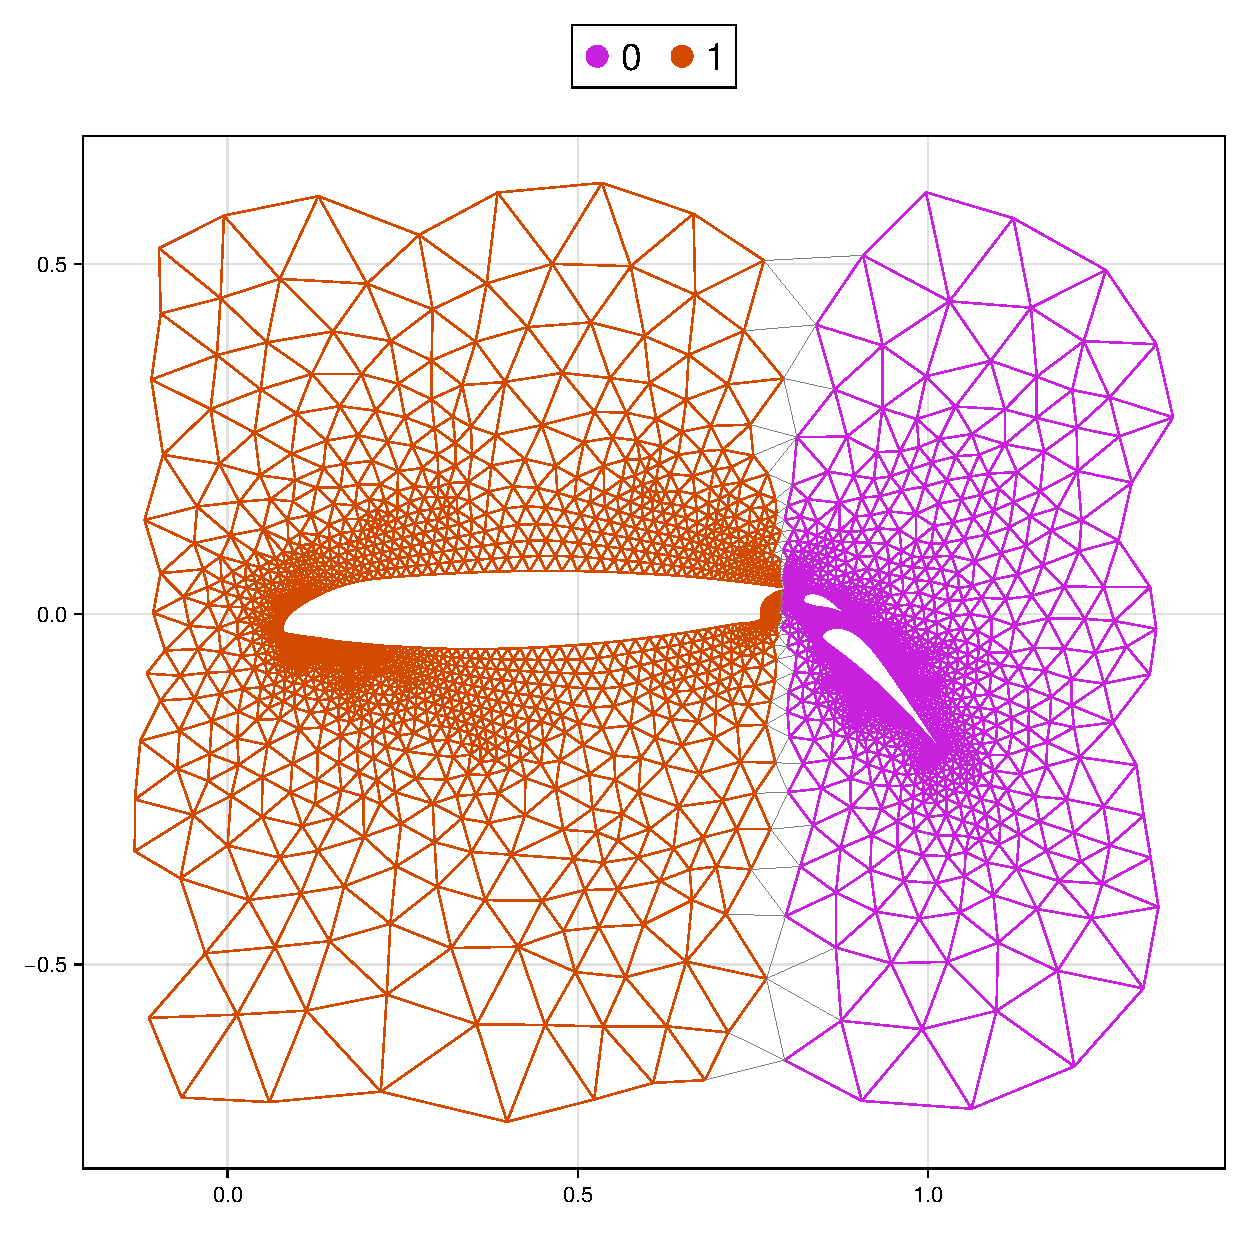
\includegraphics[width=\textwidth]{../01_graph/images/bisection/airfoil1_inertial_bisection.pdf}
    \caption{Inertial}
\end{subfigure}
\begin{subfigure}[b]{0.24\textwidth}
    \centering
    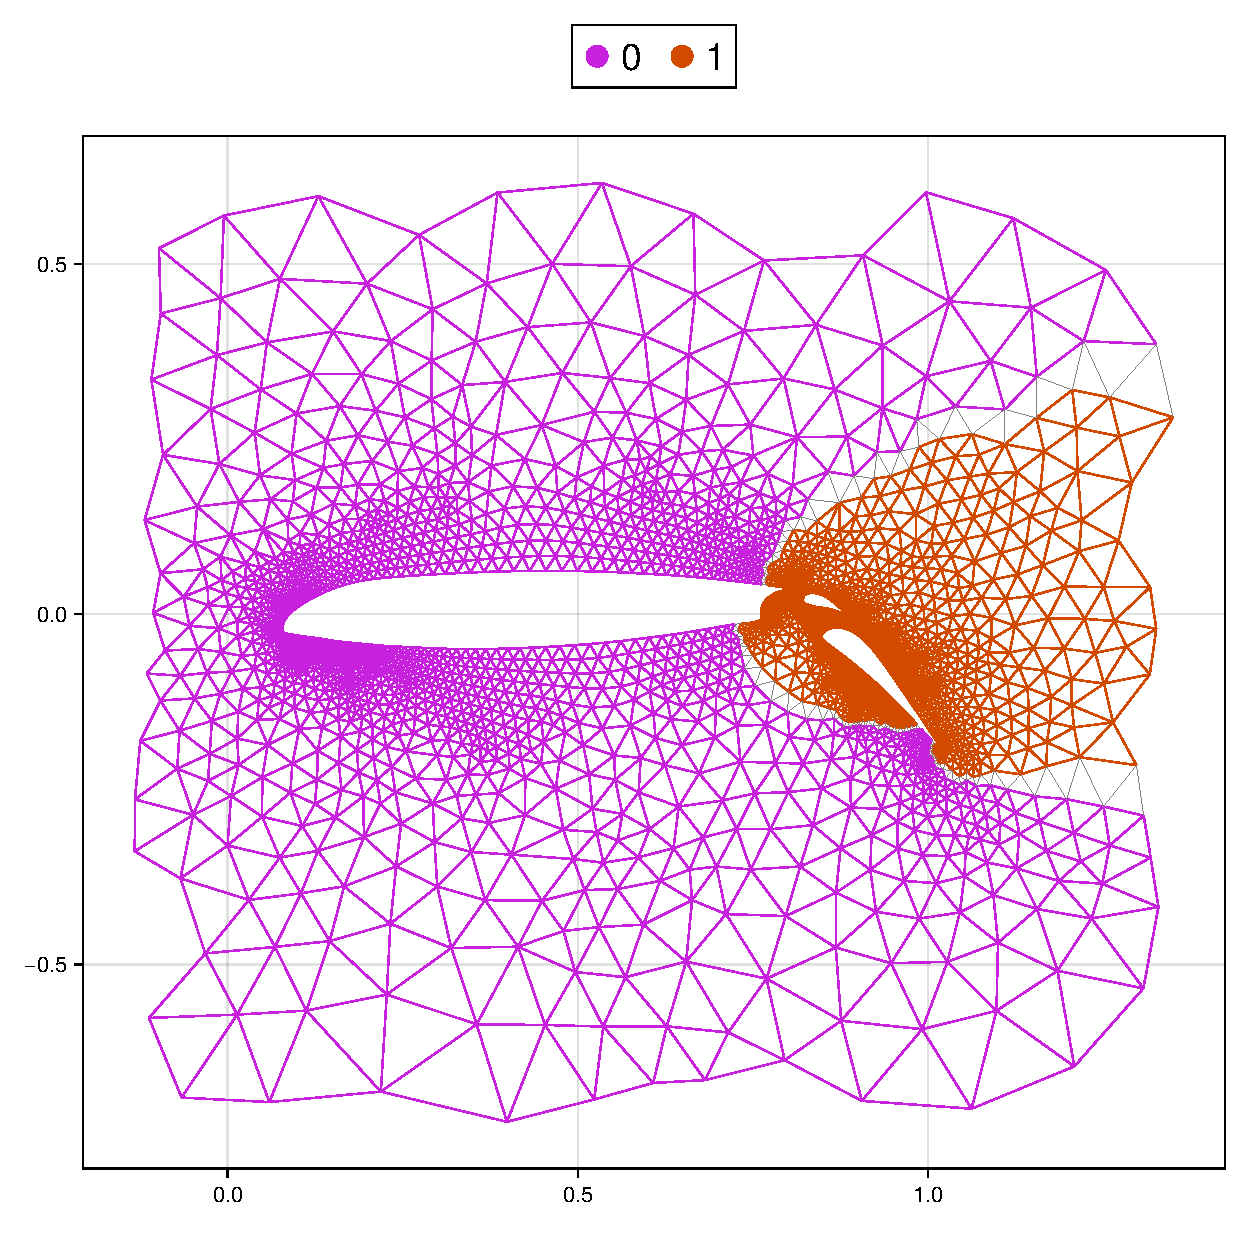
\includegraphics[width=\textwidth]{../01_graph/images/bisection/airfoil1_spectral_bisection.pdf}
    \caption{Spectral}
\end{subfigure}
\begin{subfigure}[b]{0.24\textwidth}
    \centering
    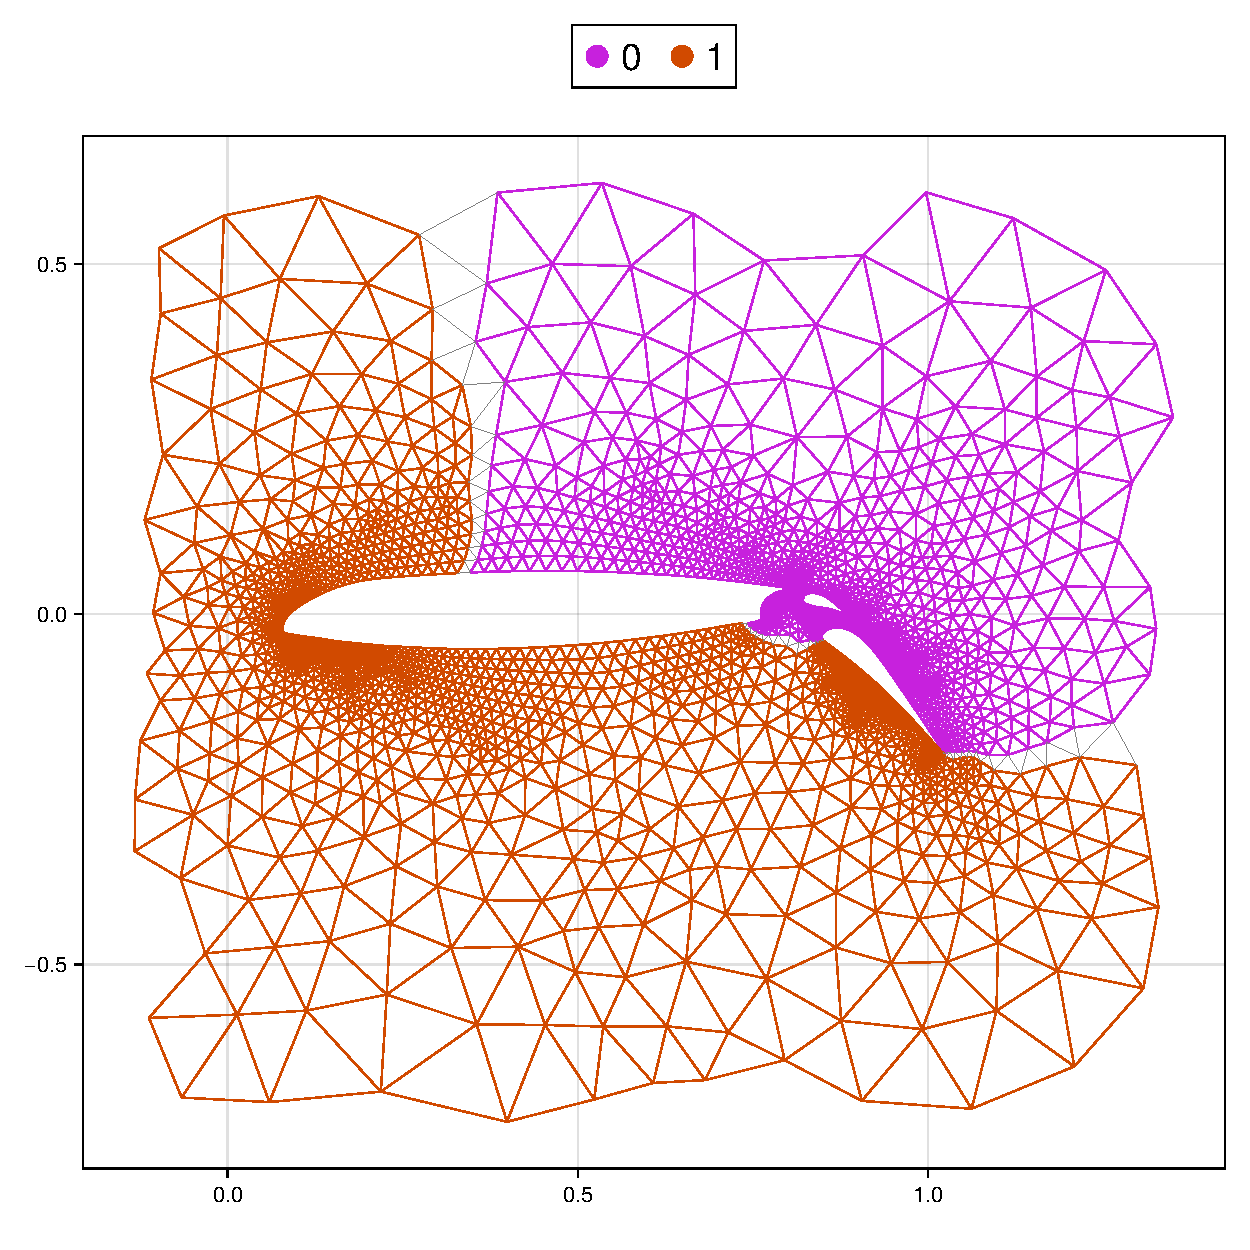
\includegraphics[width=\textwidth]{../01_graph/images/bisection/airfoil1_metis_bisection.pdf}
    \caption{METIS}
\end{subfigure}
\caption{Bisection partitions obtained for the \texttt{airfoil1} mesh.}
\label{fig:airfoil1_bisections}
\end{figure}

\begin{figure}[h]
\centering
\begin{subfigure}[b]{0.24\textwidth}
    \centering
    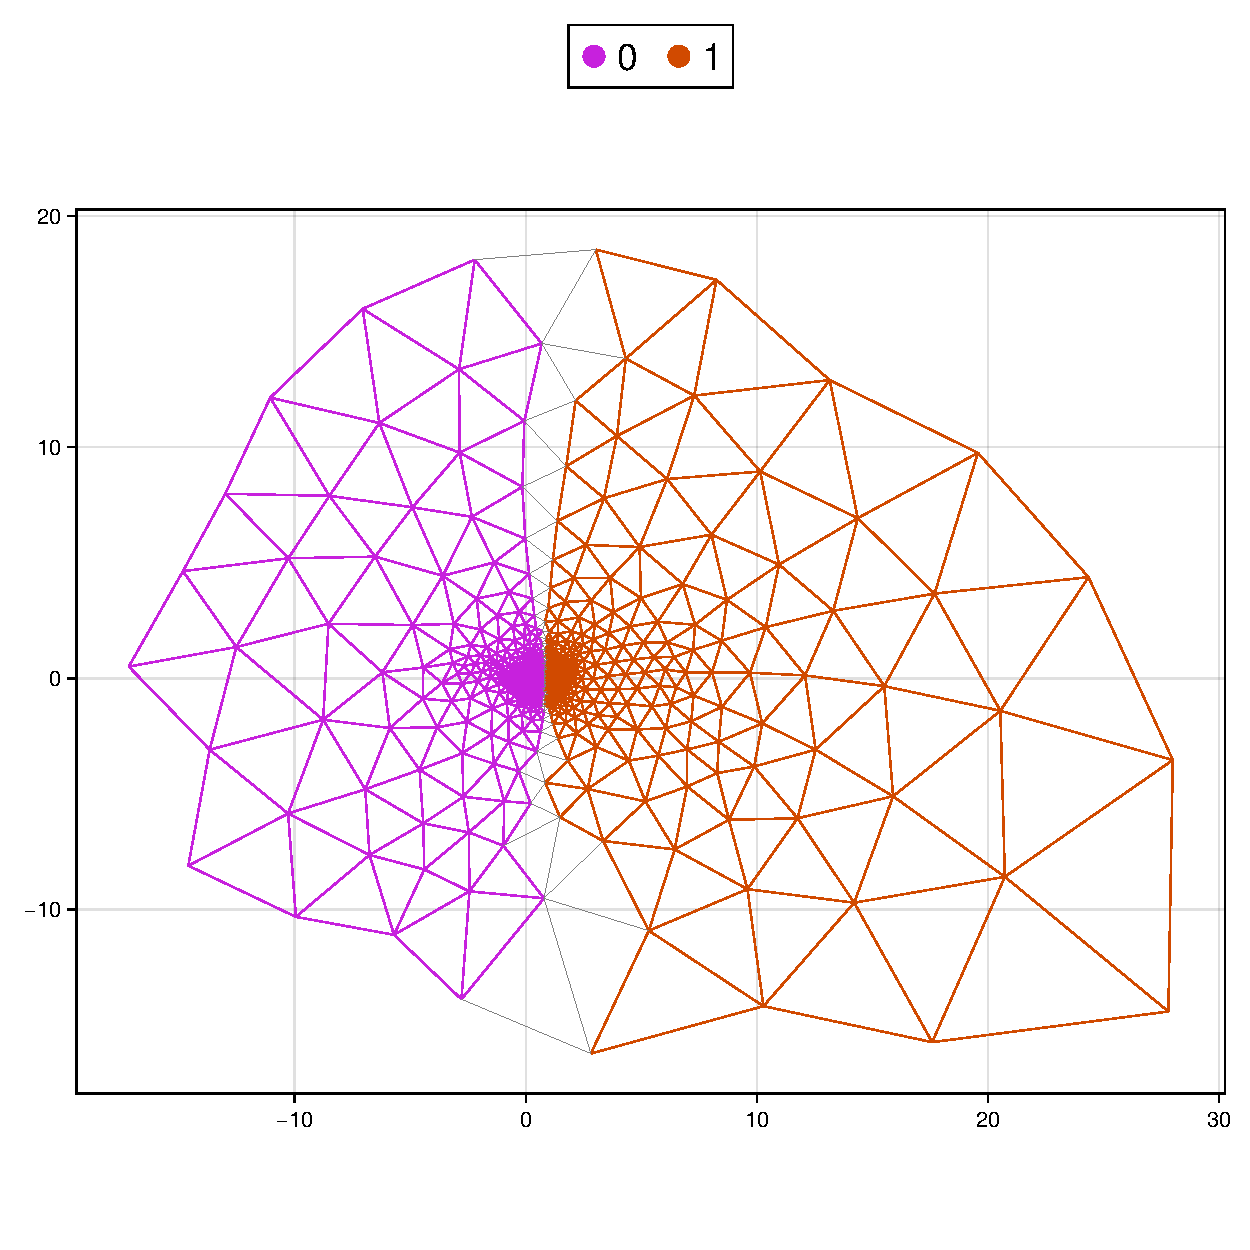
\includegraphics[width=\textwidth]{../01_graph/images/bisection/barth4_coordinate_bisection.pdf}
    \caption{Coordinate}
\end{subfigure}
\begin{subfigure}[b]{0.24\textwidth}
    \centering
    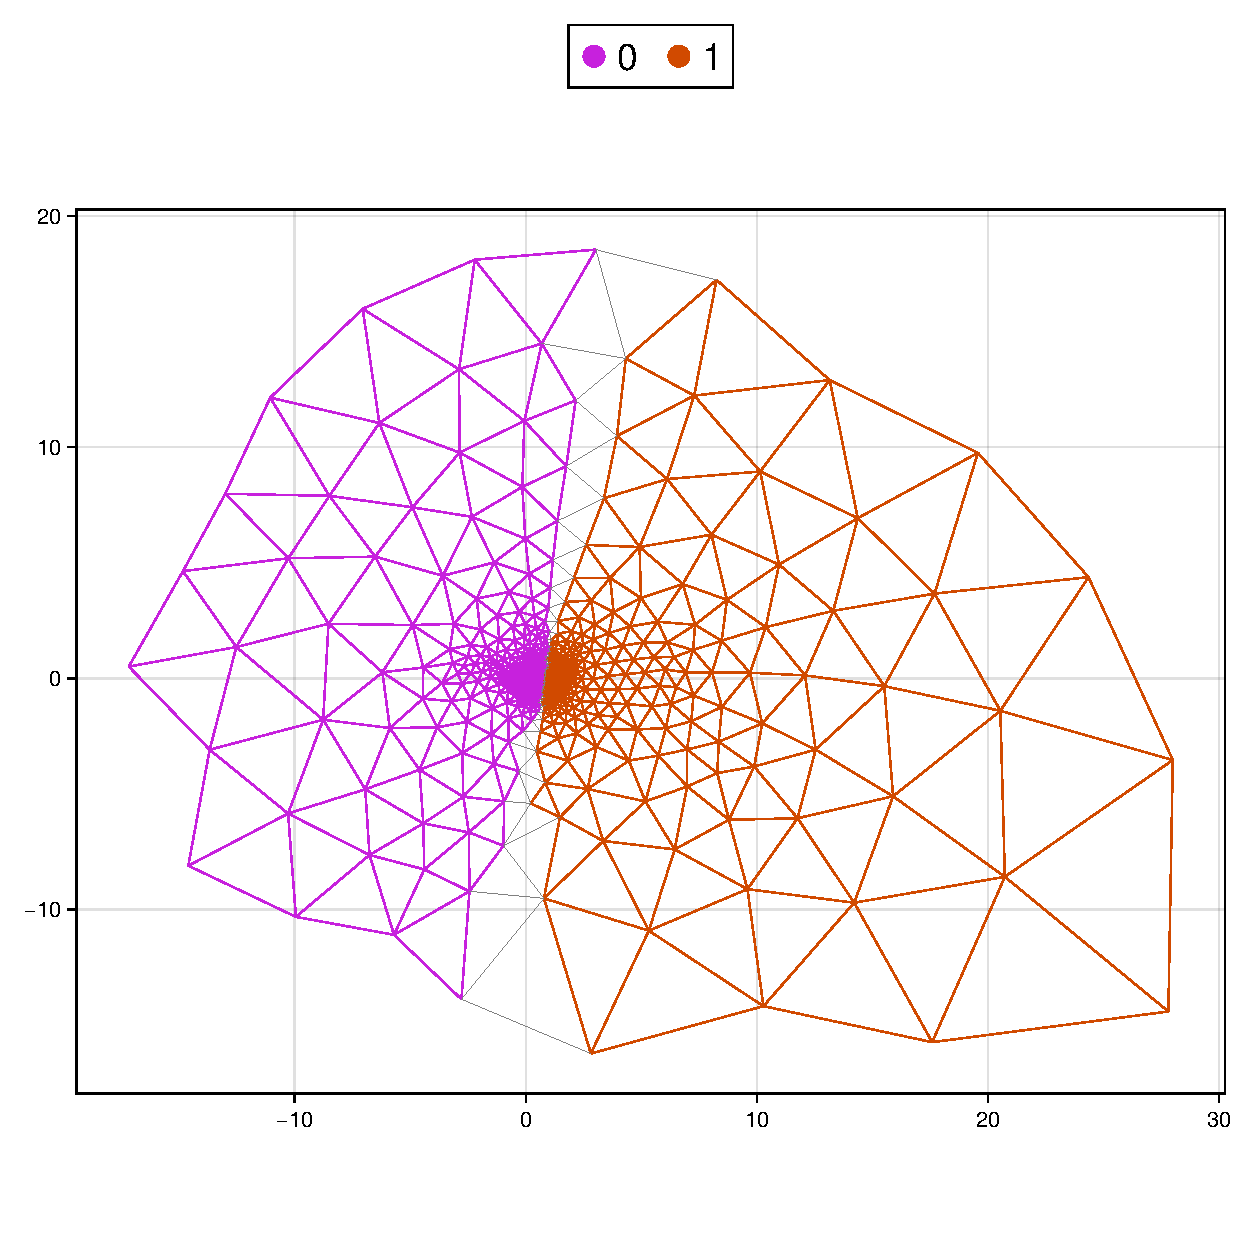
\includegraphics[width=\textwidth]{../01_graph/images/bisection/barth4_inertial_bisection.pdf}
    \caption{Inertial}
\end{subfigure}
\begin{subfigure}[b]{0.24\textwidth}
    \centering
    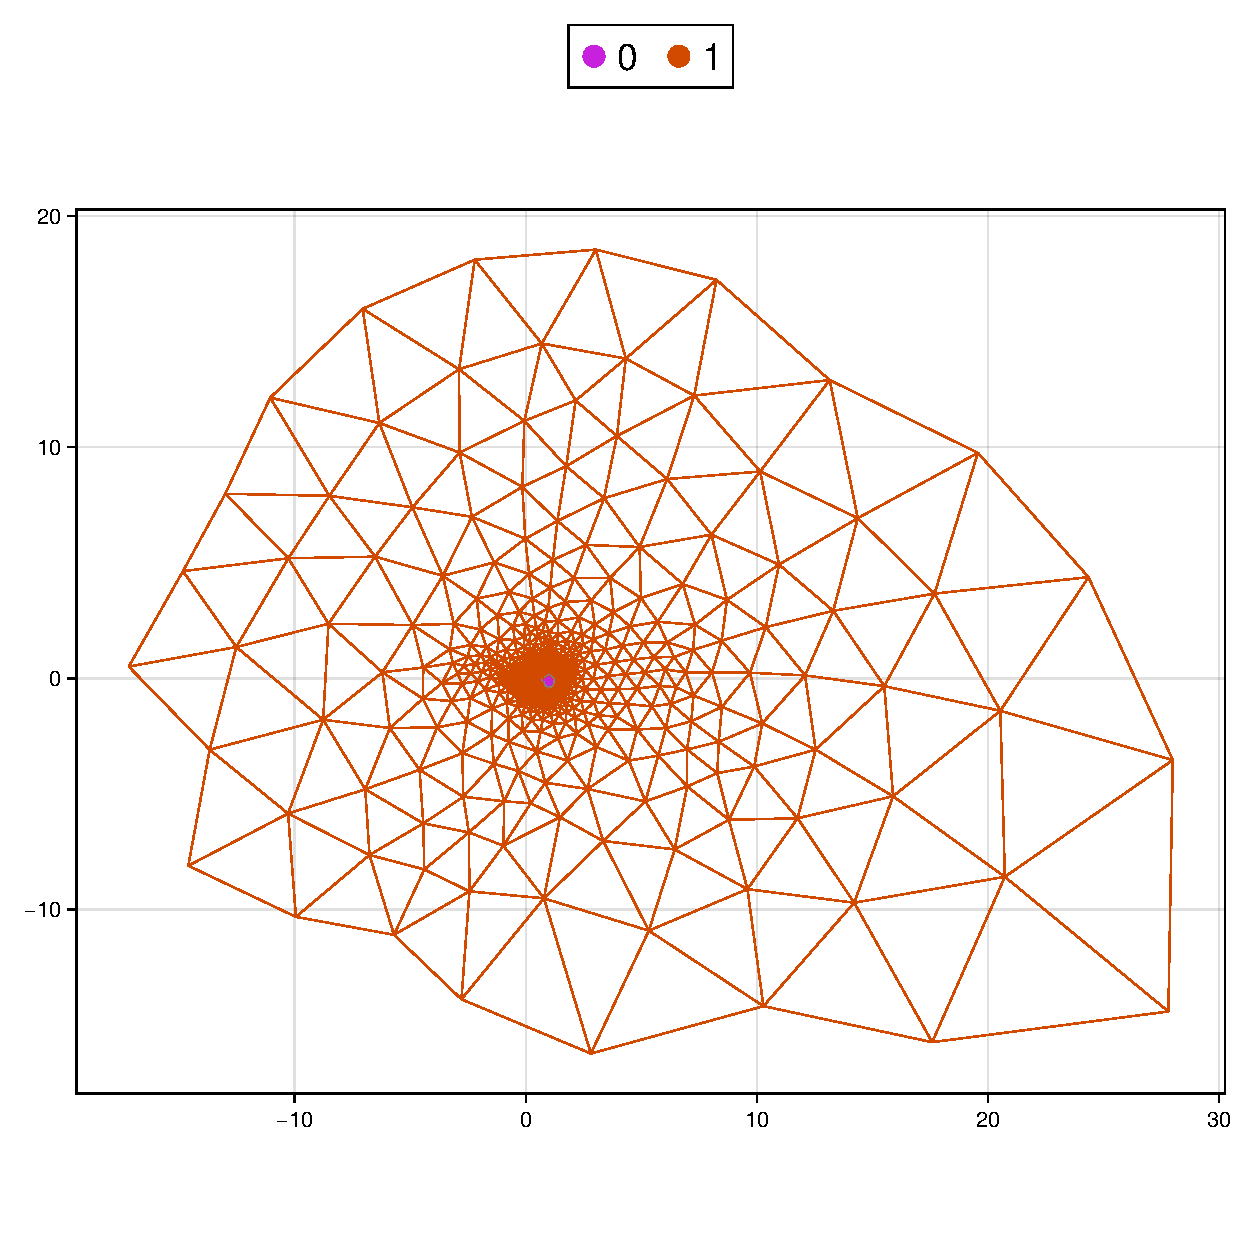
\includegraphics[width=\textwidth]{../01_graph/images/bisection/barth4_spectral_bisection.pdf}
    \caption{Spectral}
\end{subfigure}
\begin{subfigure}[b]{0.24\textwidth}
    \centering
    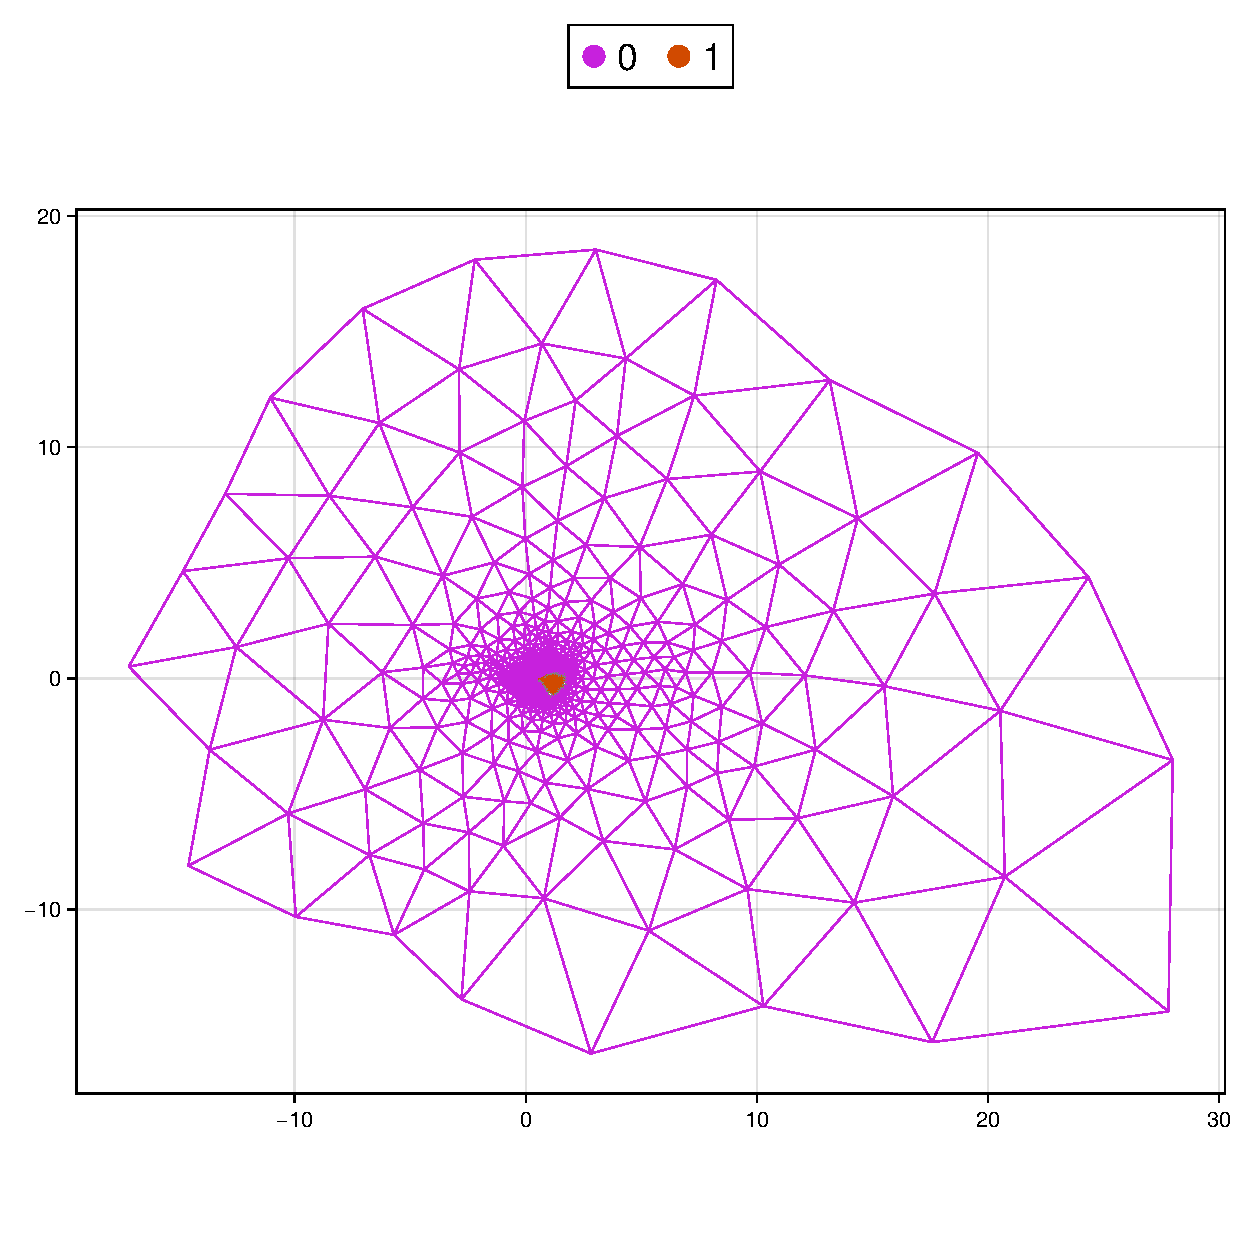
\includegraphics[width=\textwidth]{../01_graph/images/bisection/barth4_metis_bisection.pdf}
    \caption{METIS}
\end{subfigure}
\caption{Bisection partitions obtained for the \texttt{barth4} mesh.}
\label{fig:barth4_bisections}
\end{figure}

\begin{figure}[h]
\centering
\begin{subfigure}[b]{0.24\textwidth}
    \centering
    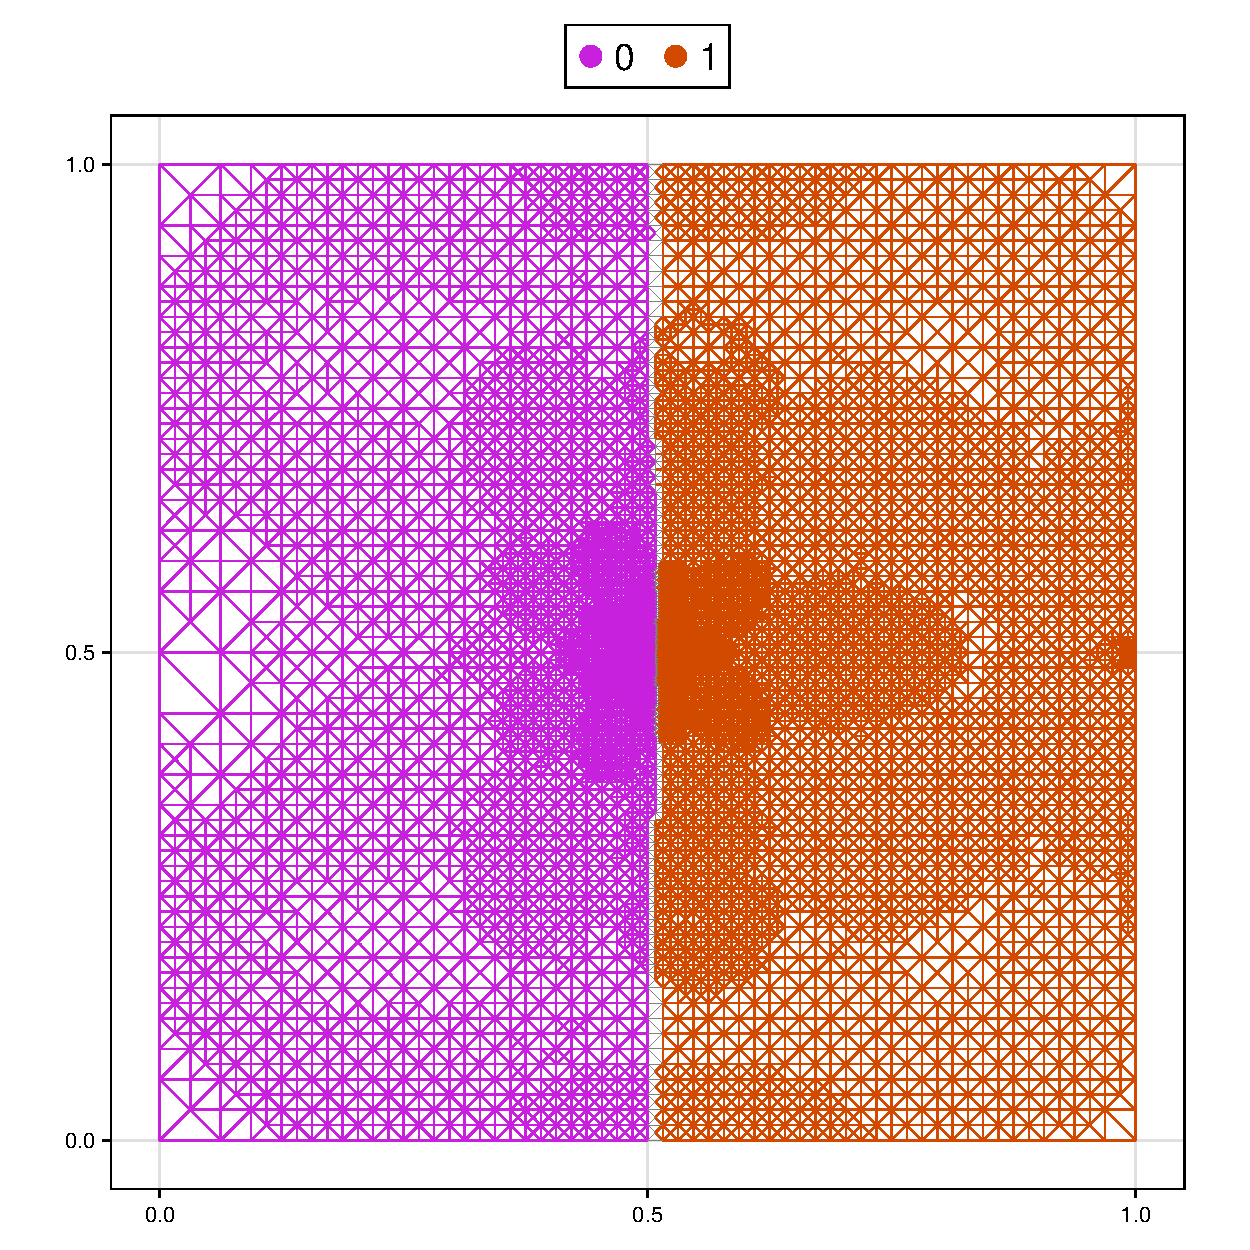
\includegraphics[width=\textwidth]{../01_graph/images/bisection/crack_coordinate_bisection.pdf}
    \caption{Coordinate}
\end{subfigure}
\begin{subfigure}[b]{0.24\textwidth}
    \centering
    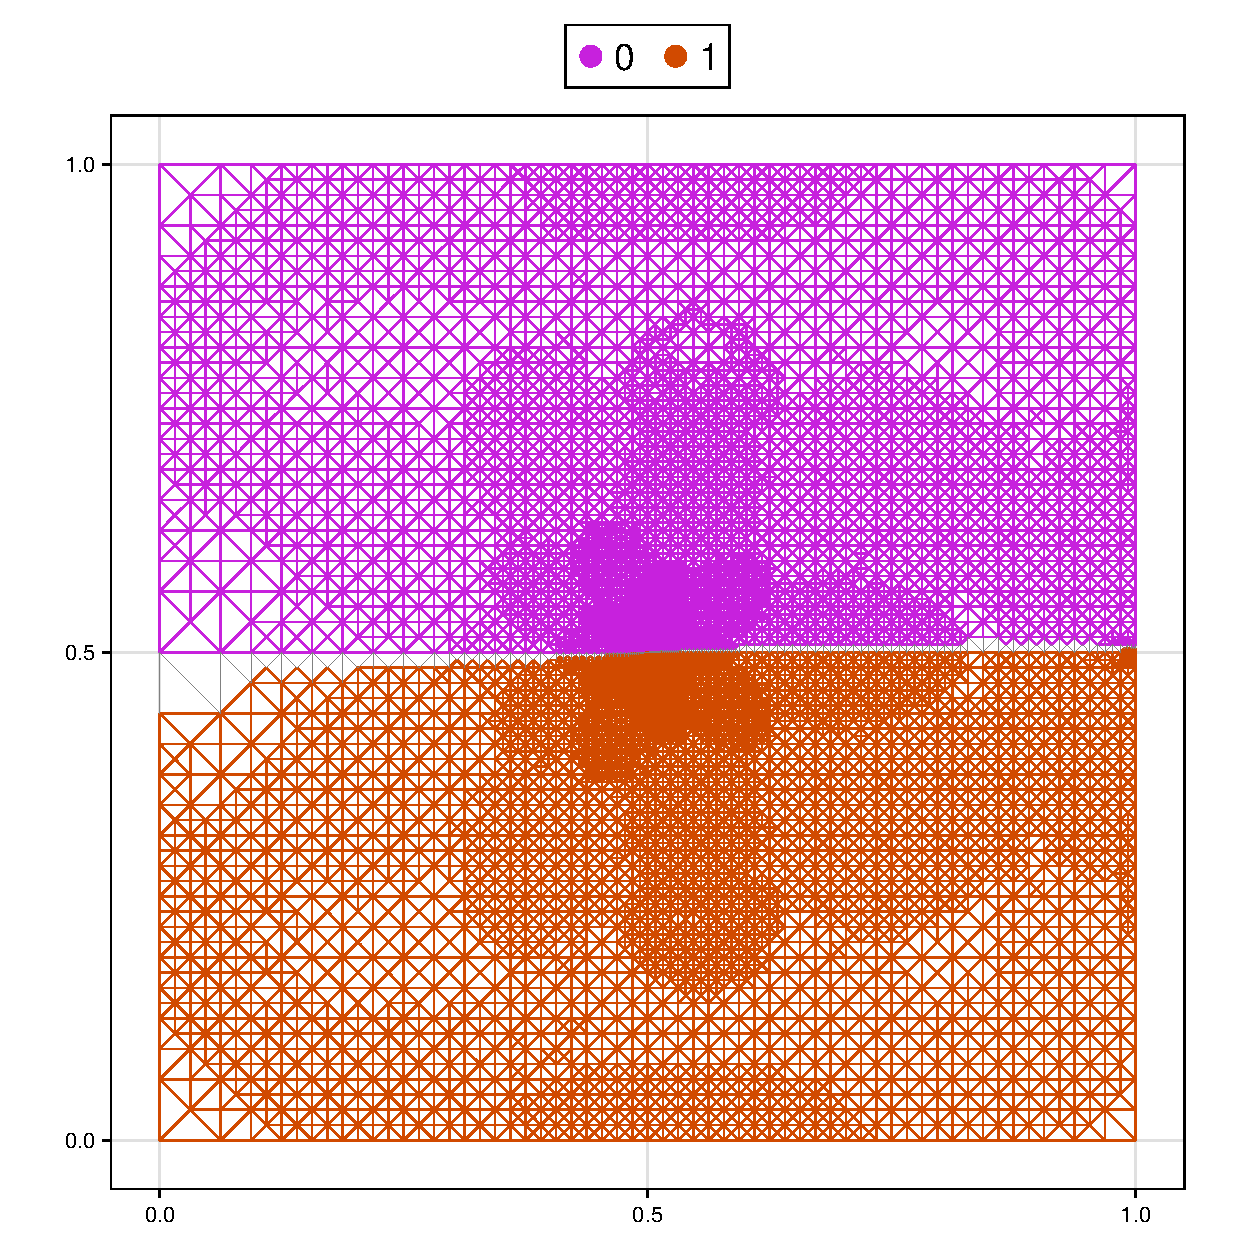
\includegraphics[width=\textwidth]{../01_graph/images/bisection/crack_inertial_bisection.pdf}
    \caption{Inertial}
\end{subfigure}
\begin{subfigure}[b]{0.24\textwidth}
    \centering
    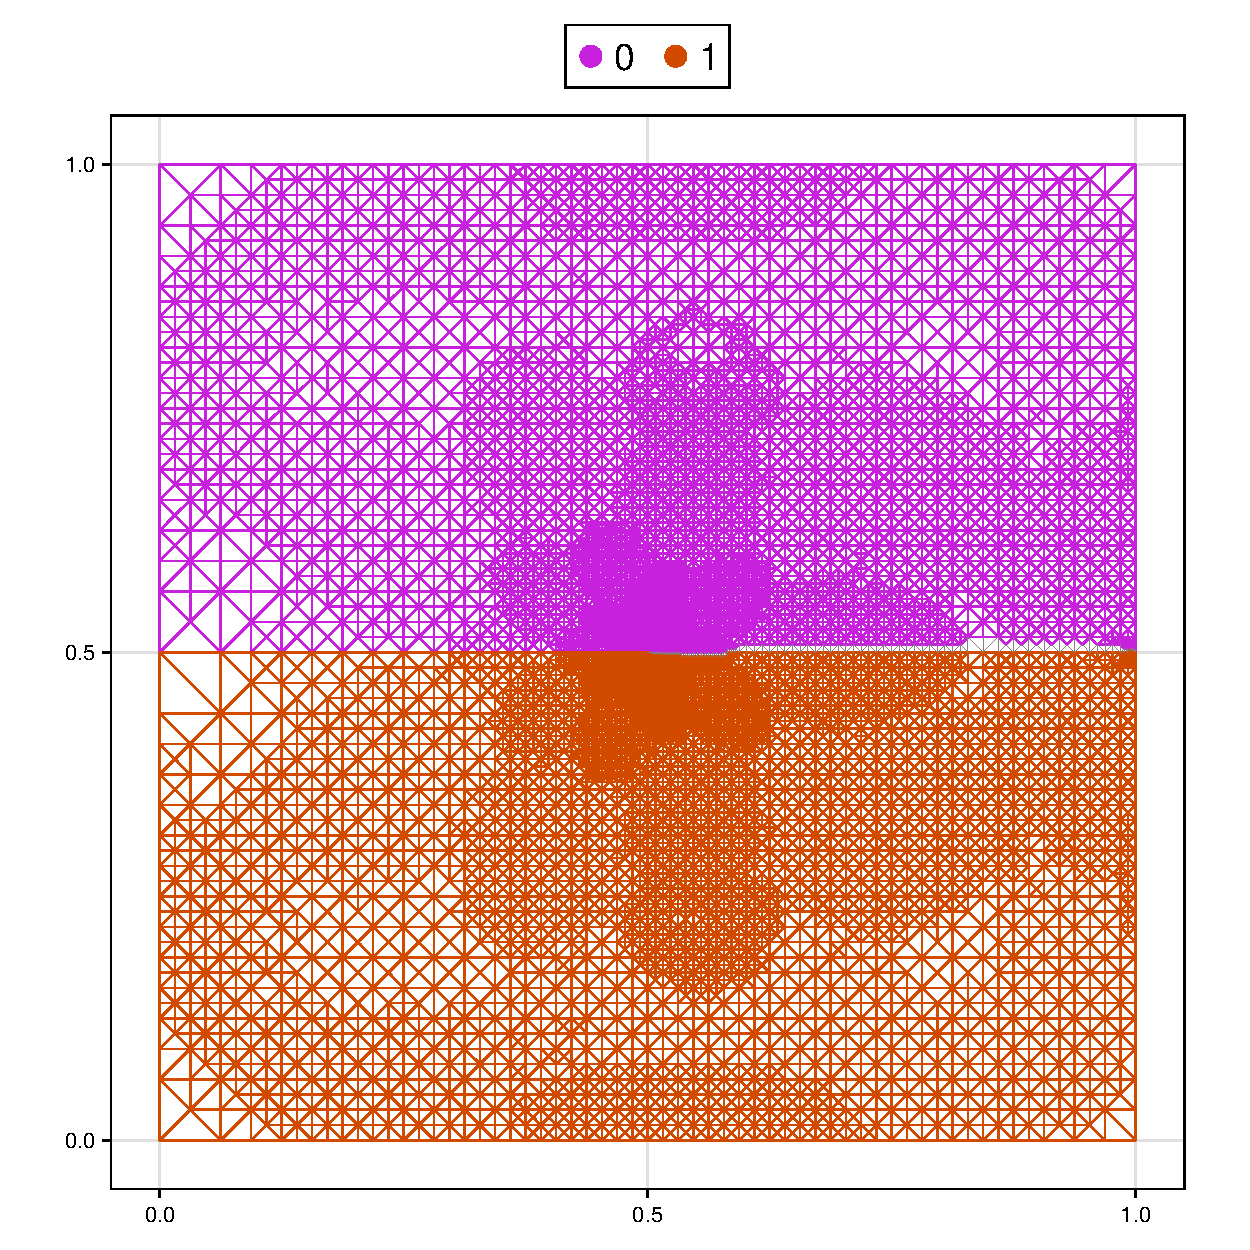
\includegraphics[width=\textwidth]{../01_graph/images/bisection/crack_spectral_bisection.pdf}
    \caption{Spectral}
\end{subfigure}
\begin{subfigure}[b]{0.24\textwidth}
    \centering
    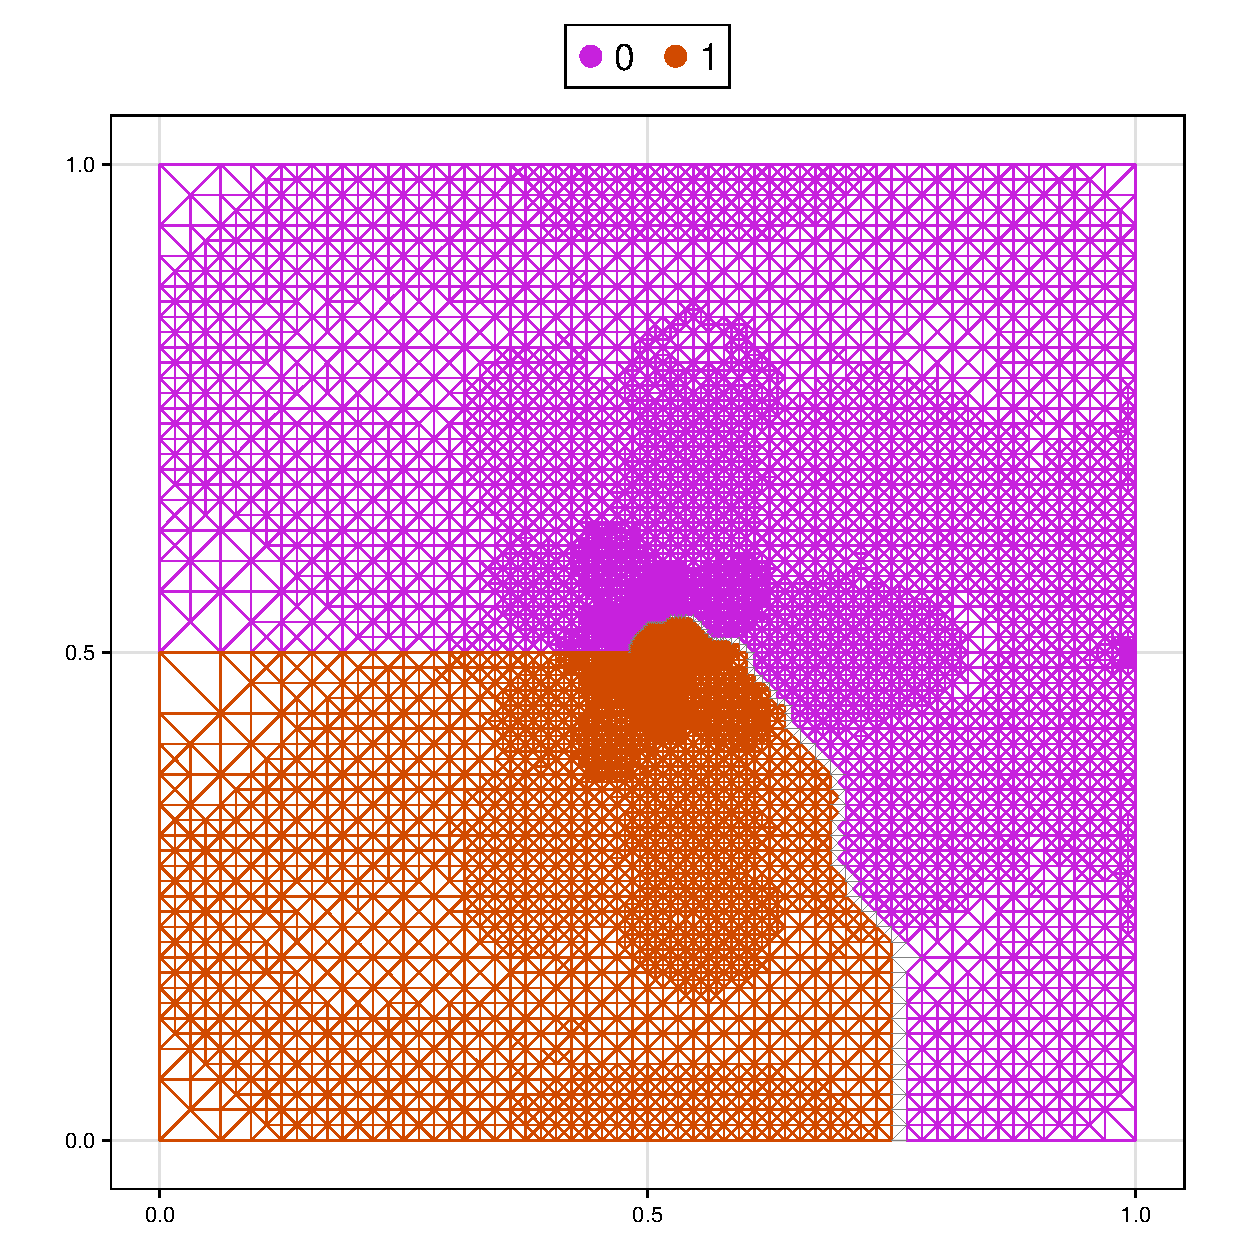
\includegraphics[width=\textwidth]{../01_graph/images/bisection/crack_metis_bisection.pdf}
    \caption{METIS}
\end{subfigure}
\caption{Bisection partitions obtained for the \texttt{crack} mesh.}
\label{fig:crack_bisections}
\end{figure}

\begin{figure}[h]
\centering
\begin{subfigure}[b]{0.24\textwidth}
    \centering
    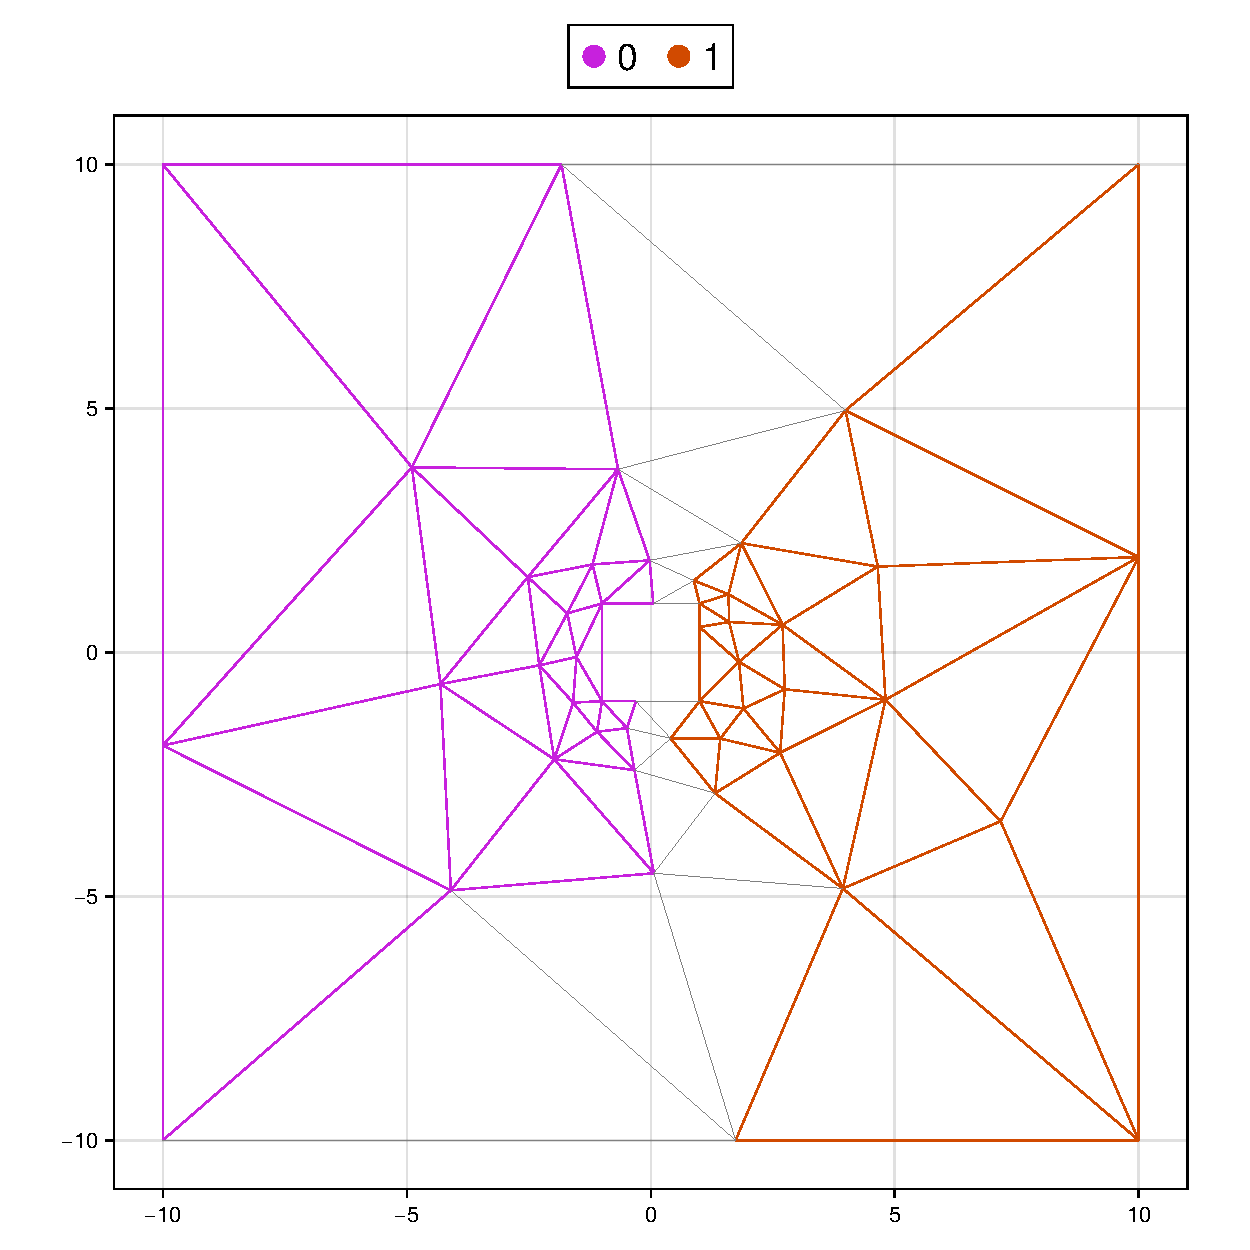
\includegraphics[width=\textwidth]{../01_graph/images/bisection/mesh1e1_coordinate_bisection.pdf}
    \caption{Coordinate}
\end{subfigure}
\begin{subfigure}[b]{0.24\textwidth}
    \centering
    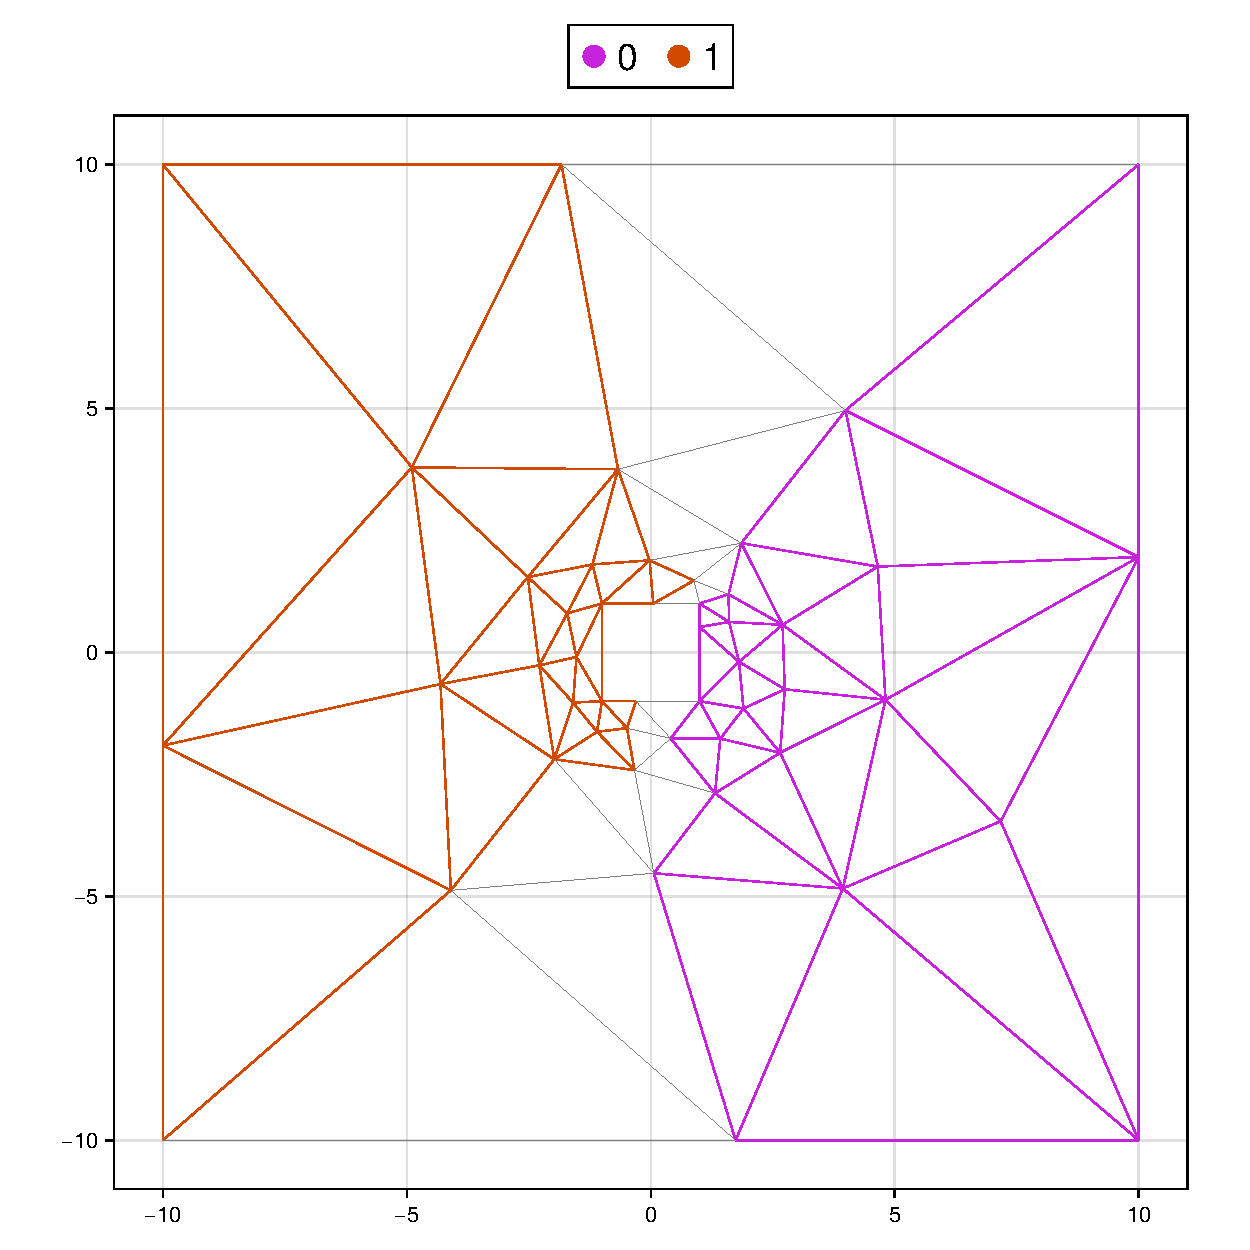
\includegraphics[width=\textwidth]{../01_graph/images/bisection/mesh1e1_inertial_bisection.pdf}
    \caption{Inertial}
\end{subfigure}
\begin{subfigure}[b]{0.24\textwidth}
    \centering
    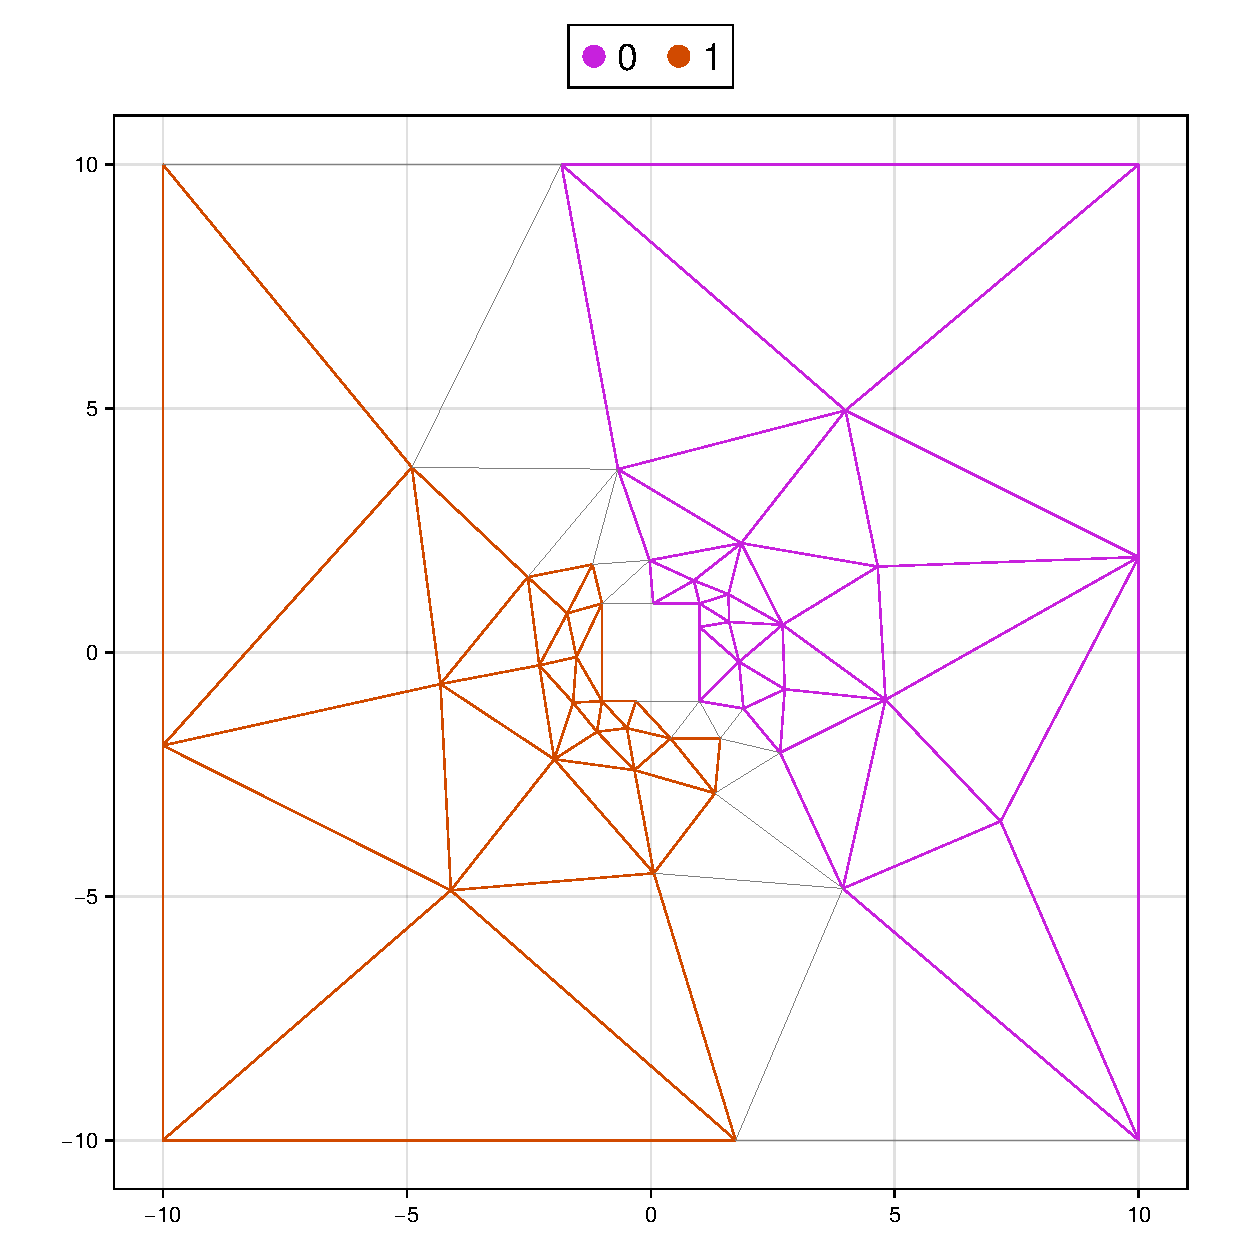
\includegraphics[width=\textwidth]{../01_graph/images/bisection/mesh1e1_spectral_bisection.pdf}
    \caption{Spectral}
\end{subfigure}
\begin{subfigure}[b]{0.24\textwidth}
    \centering
    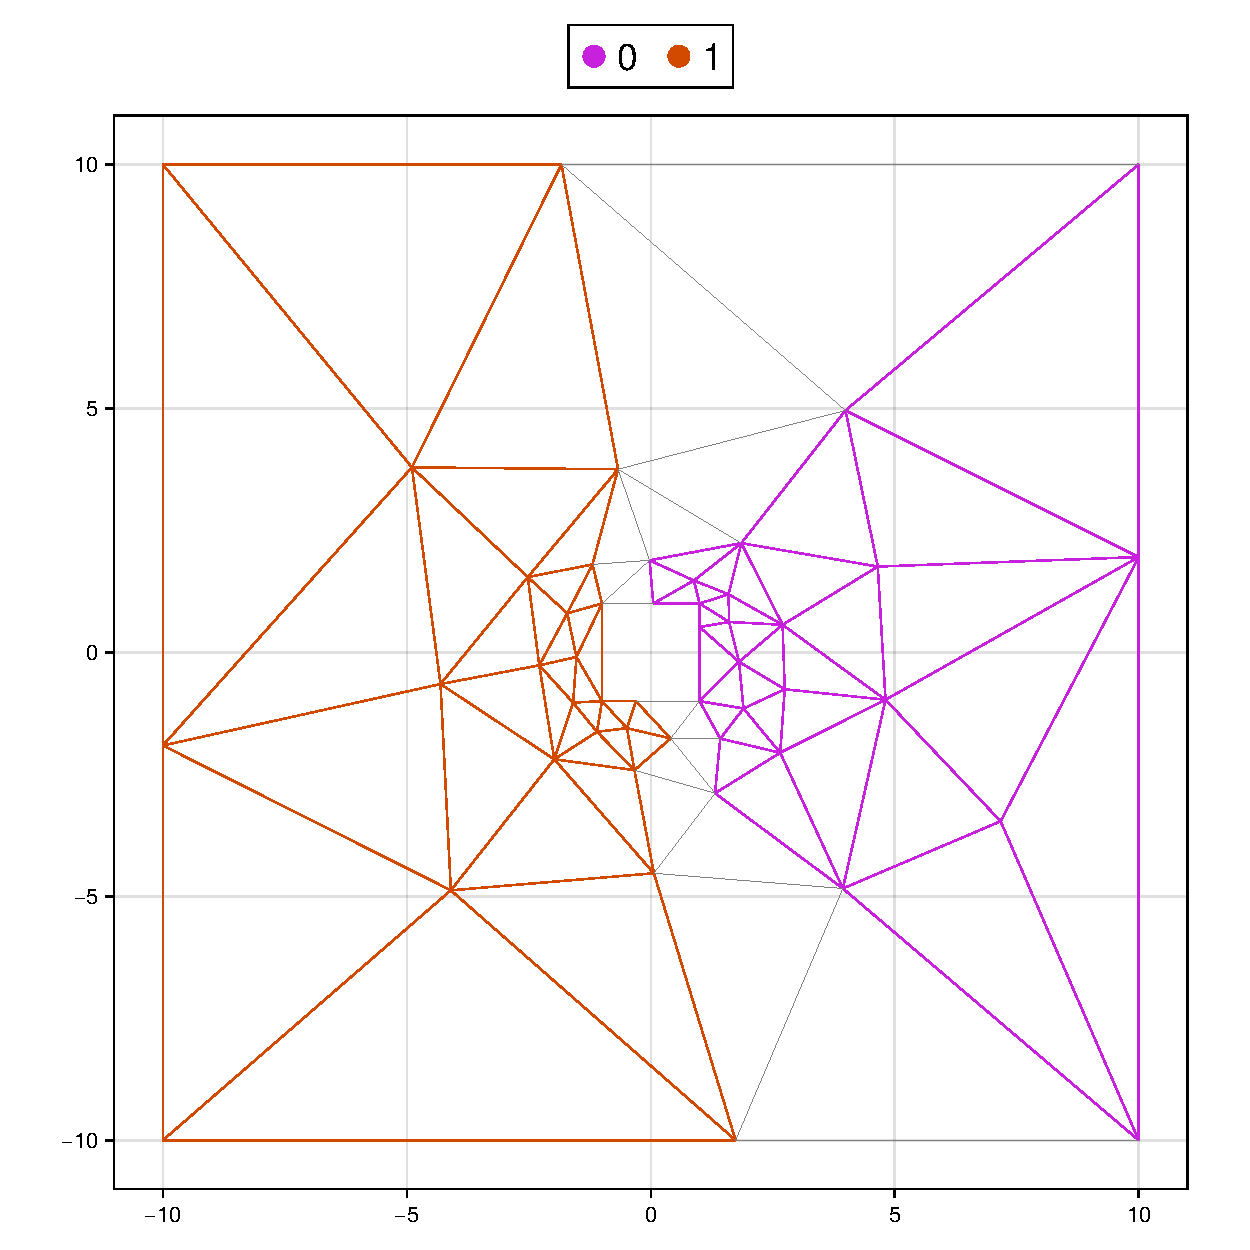
\includegraphics[width=\textwidth]{../01_graph/images/bisection/mesh1e1_metis_bisection.pdf}
    \caption{METIS}
\end{subfigure}
\caption{Bisection partitions obtained for the \texttt{mesh1e1} mesh.}
\label{fig:mesh1e1_bisections}
\end{figure}

\begin{figure}[h]
\centering
\begin{subfigure}[b]{0.24\textwidth}
    \centering
    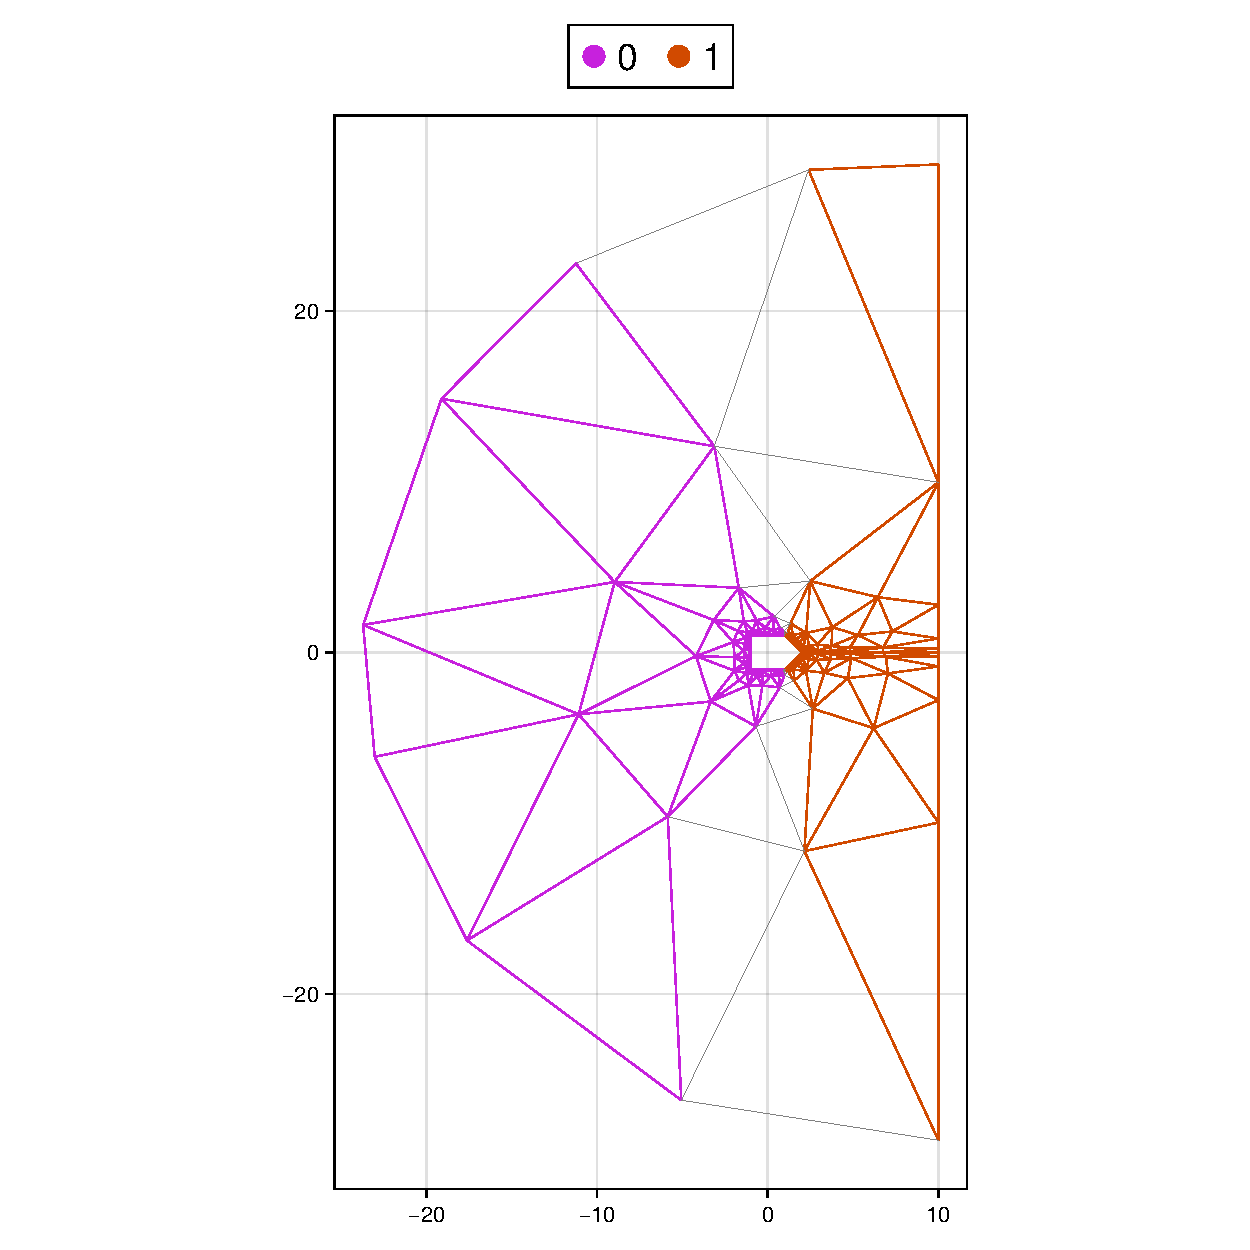
\includegraphics[width=\textwidth]{../01_graph/images/bisection/mesh2e1_coordinate_bisection.pdf}
    \caption{Coordinate}
\end{subfigure}
\begin{subfigure}[b]{0.24\textwidth}
    \centering
    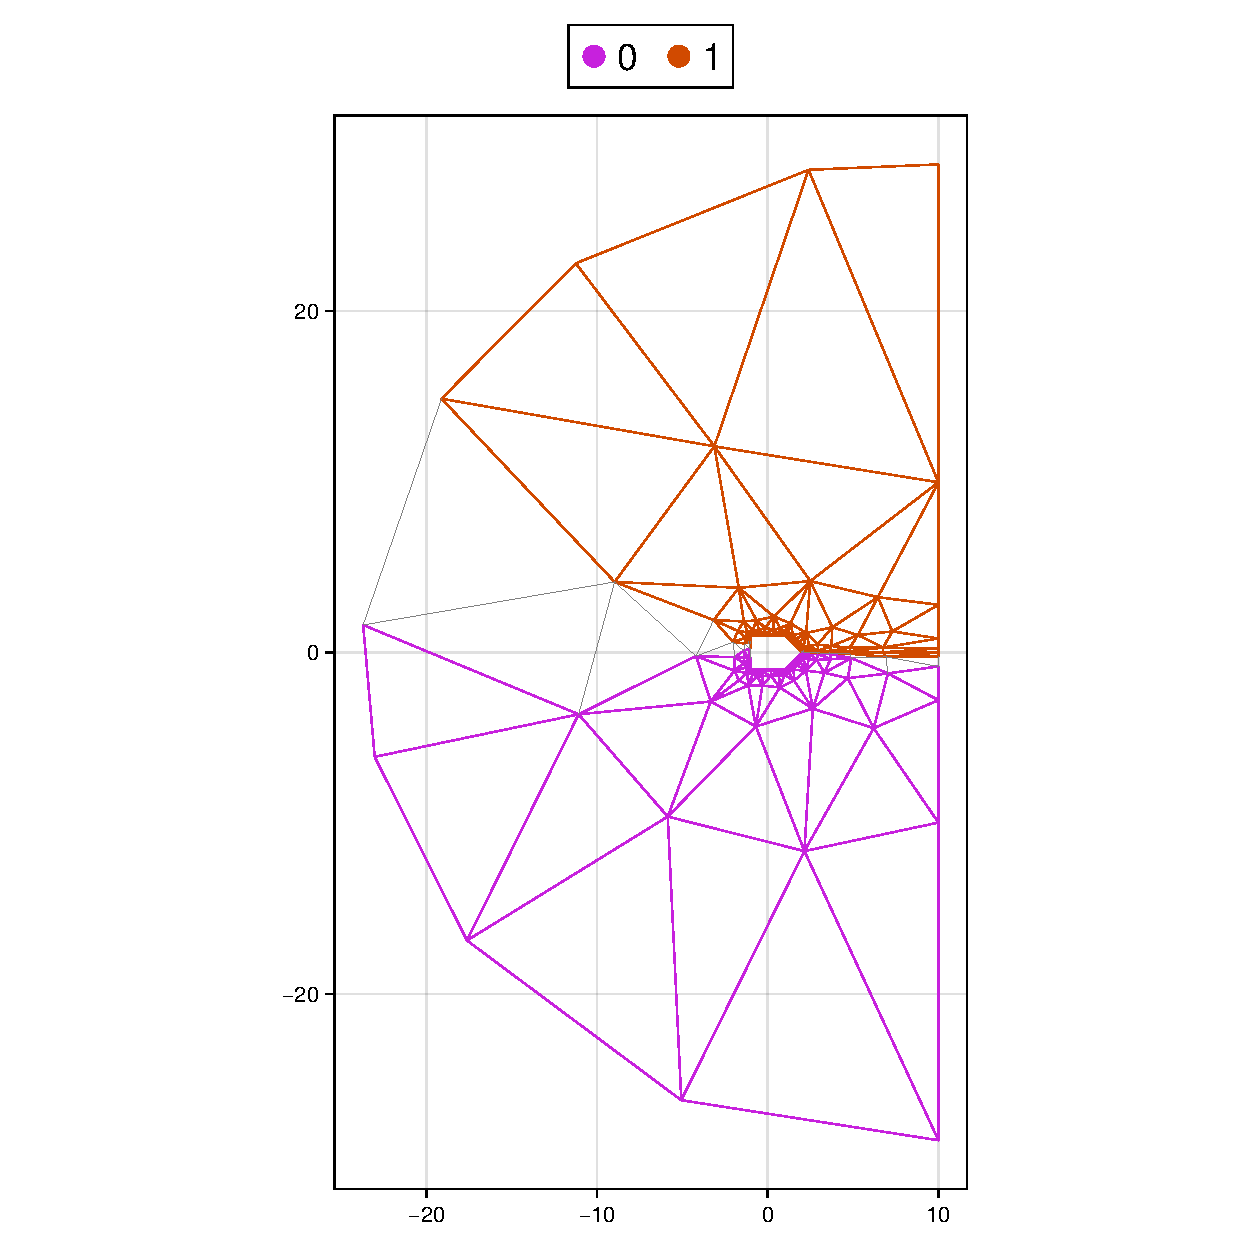
\includegraphics[width=\textwidth]{../01_graph/images/bisection/mesh2e1_inertial_bisection.pdf}
    \caption{Inertial}
\end{subfigure}
\begin{subfigure}[b]{0.24\textwidth}
    \centering
    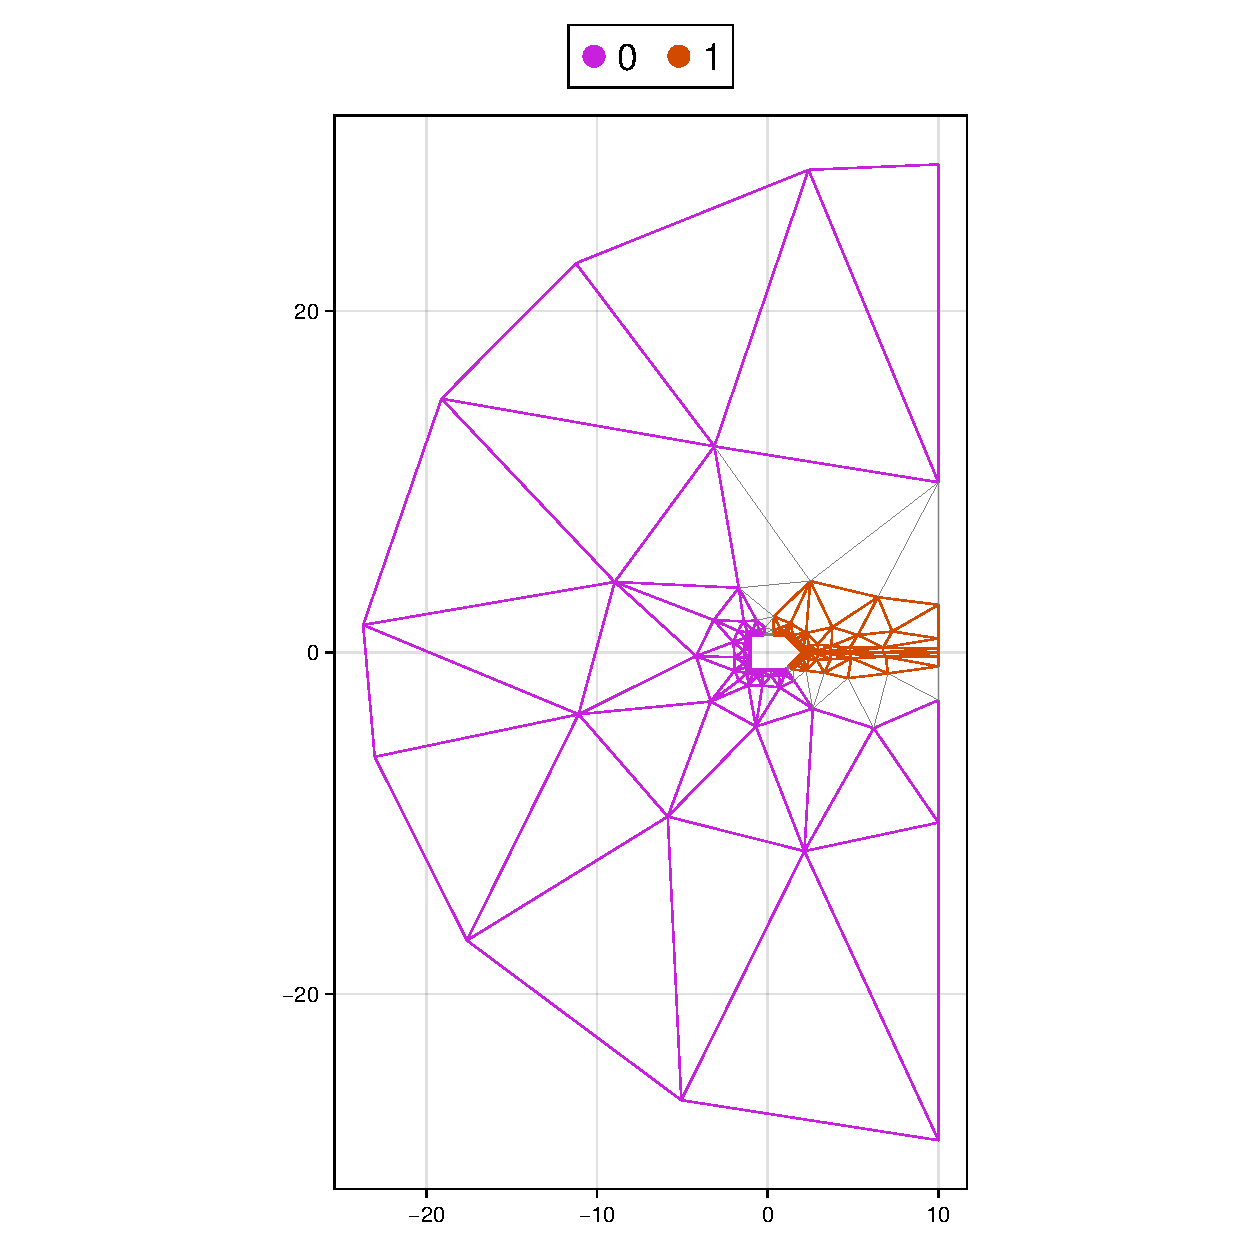
\includegraphics[width=\textwidth]{../01_graph/images/bisection/mesh2e1_spectral_bisection.pdf}
    \caption{Spectral}
\end{subfigure}
\begin{subfigure}[b]{0.24\textwidth}
    \centering
    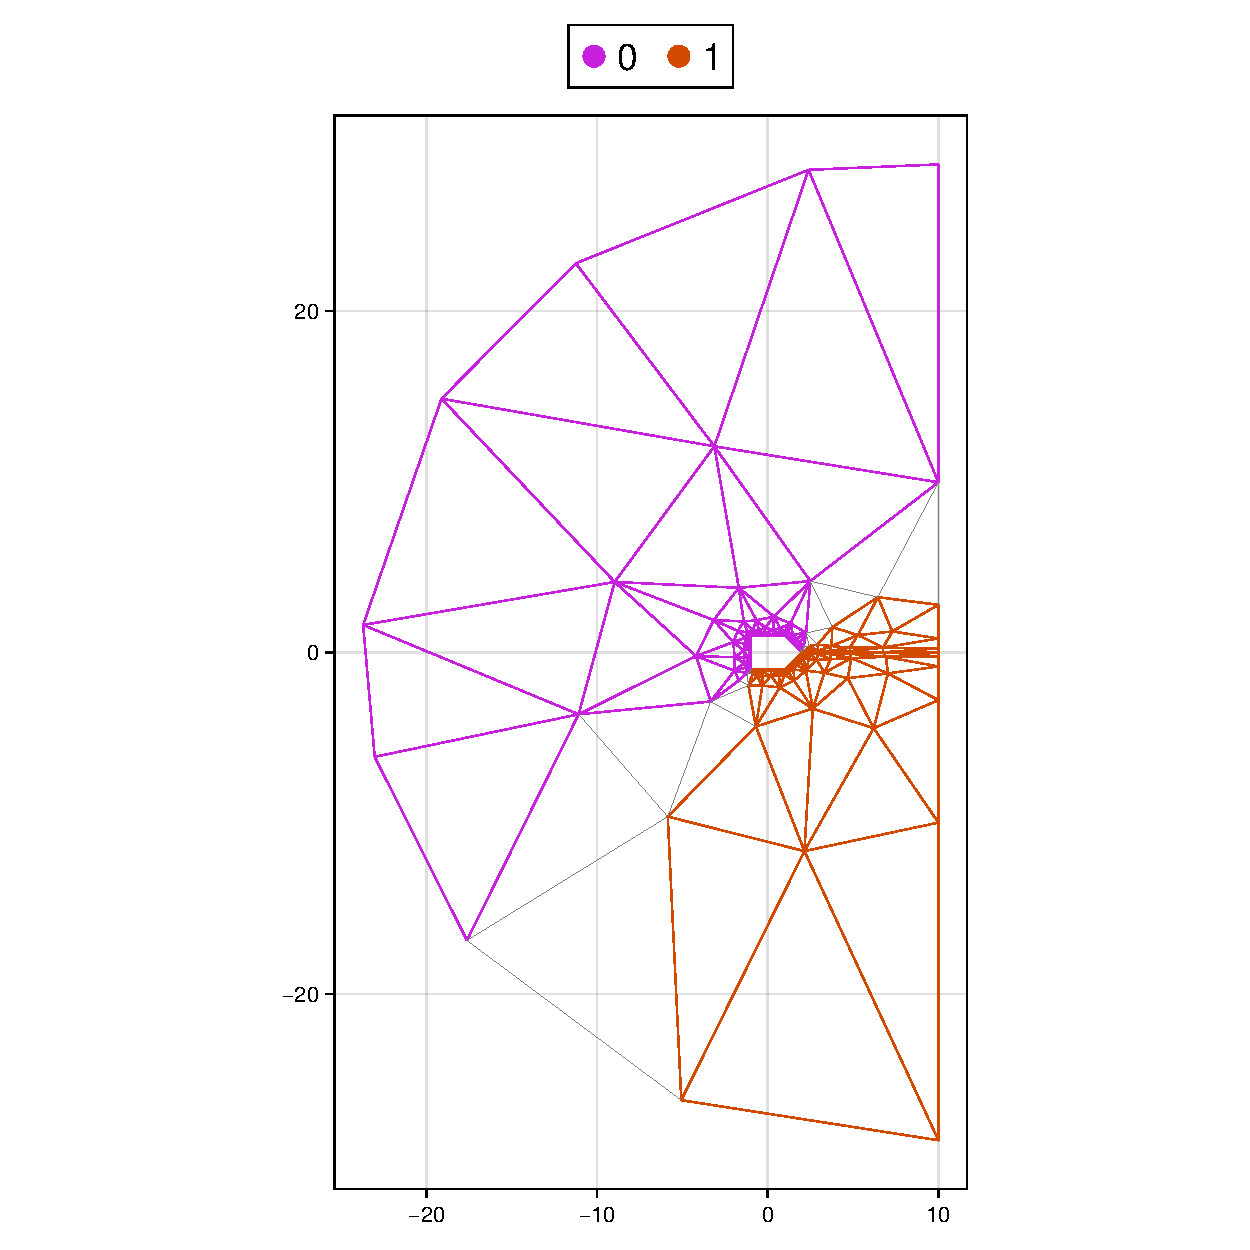
\includegraphics[width=\textwidth]{../01_graph/images/bisection/mesh2e1_metis_bisection.pdf}
    \caption{METIS}
\end{subfigure}
\caption{Bisection partitions obtained for the \texttt{mesh2e1} mesh.}
\label{fig:mesh2e1_bisections}
\end{figure}

\begin{figure}[h]
\centering
\begin{subfigure}[b]{0.24\textwidth}
    \centering
    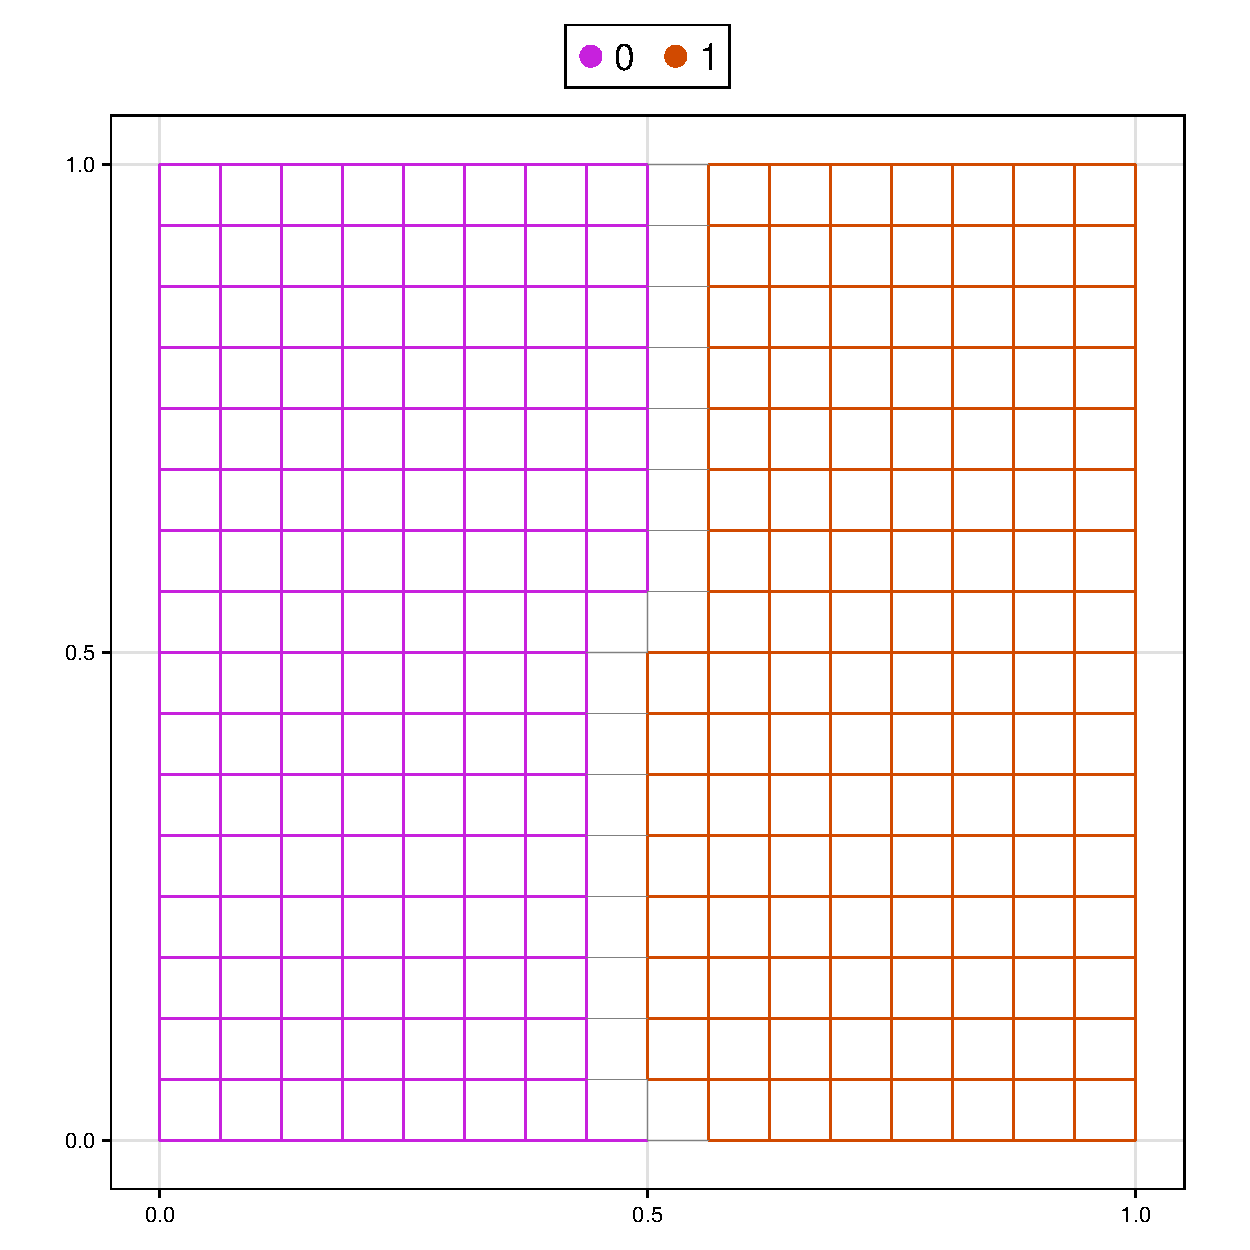
\includegraphics[width=\textwidth]{../01_graph/images/bisection/mesh3e1_coordinate_bisection.pdf}
    \caption{Coordinate}
\end{subfigure}
\begin{subfigure}[b]{0.24\textwidth}
    \centering
    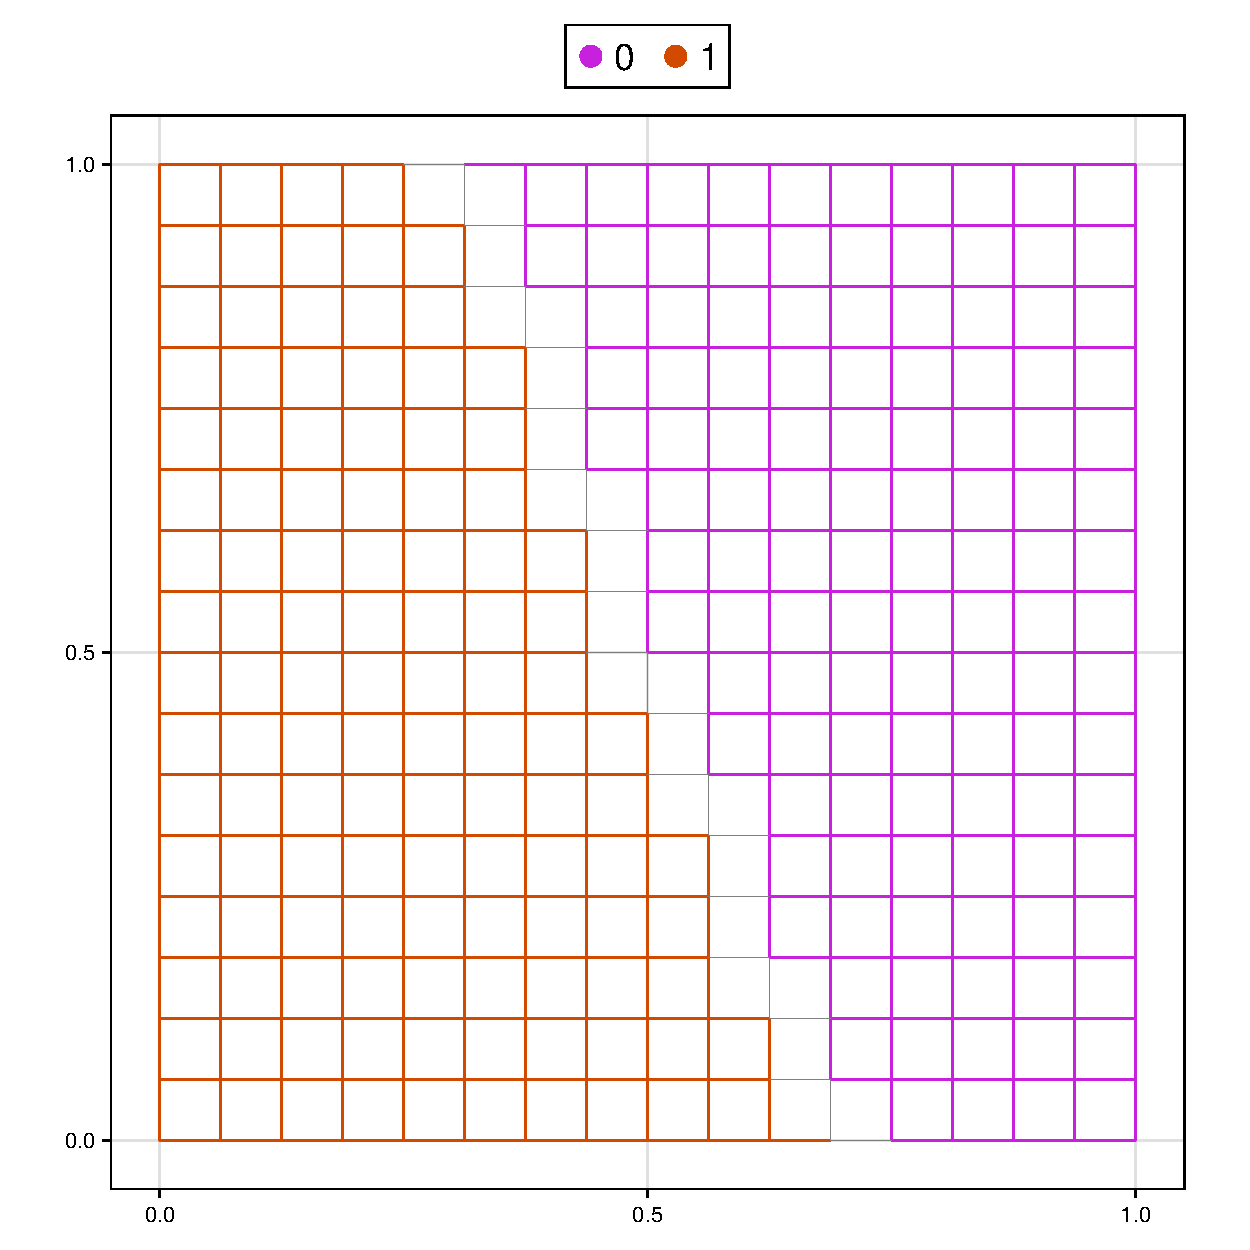
\includegraphics[width=\textwidth]{../01_graph/images/bisection/mesh3e1_inertial_bisection.pdf}
    \caption{Inertial}
\end{subfigure}
\begin{subfigure}[b]{0.24\textwidth}
    \centering
    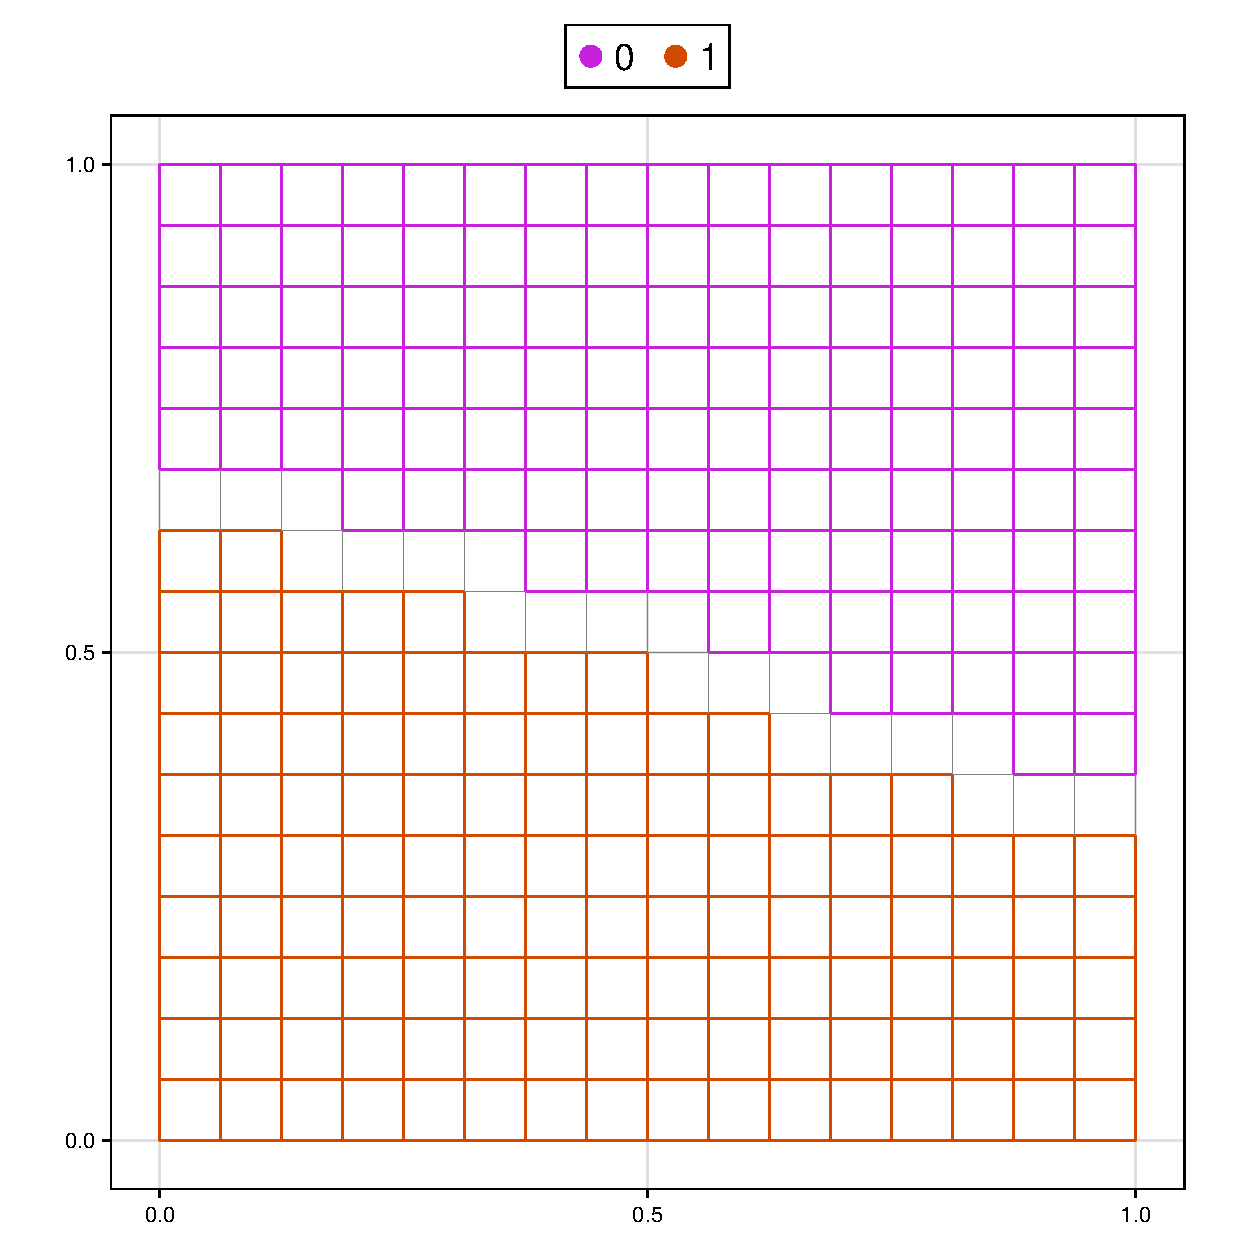
\includegraphics[width=\textwidth]{../01_graph/images/bisection/mesh3e1_spectral_bisection.pdf}
    \caption{Spectral}
\end{subfigure}
\begin{subfigure}[b]{0.24\textwidth}
    \centering
    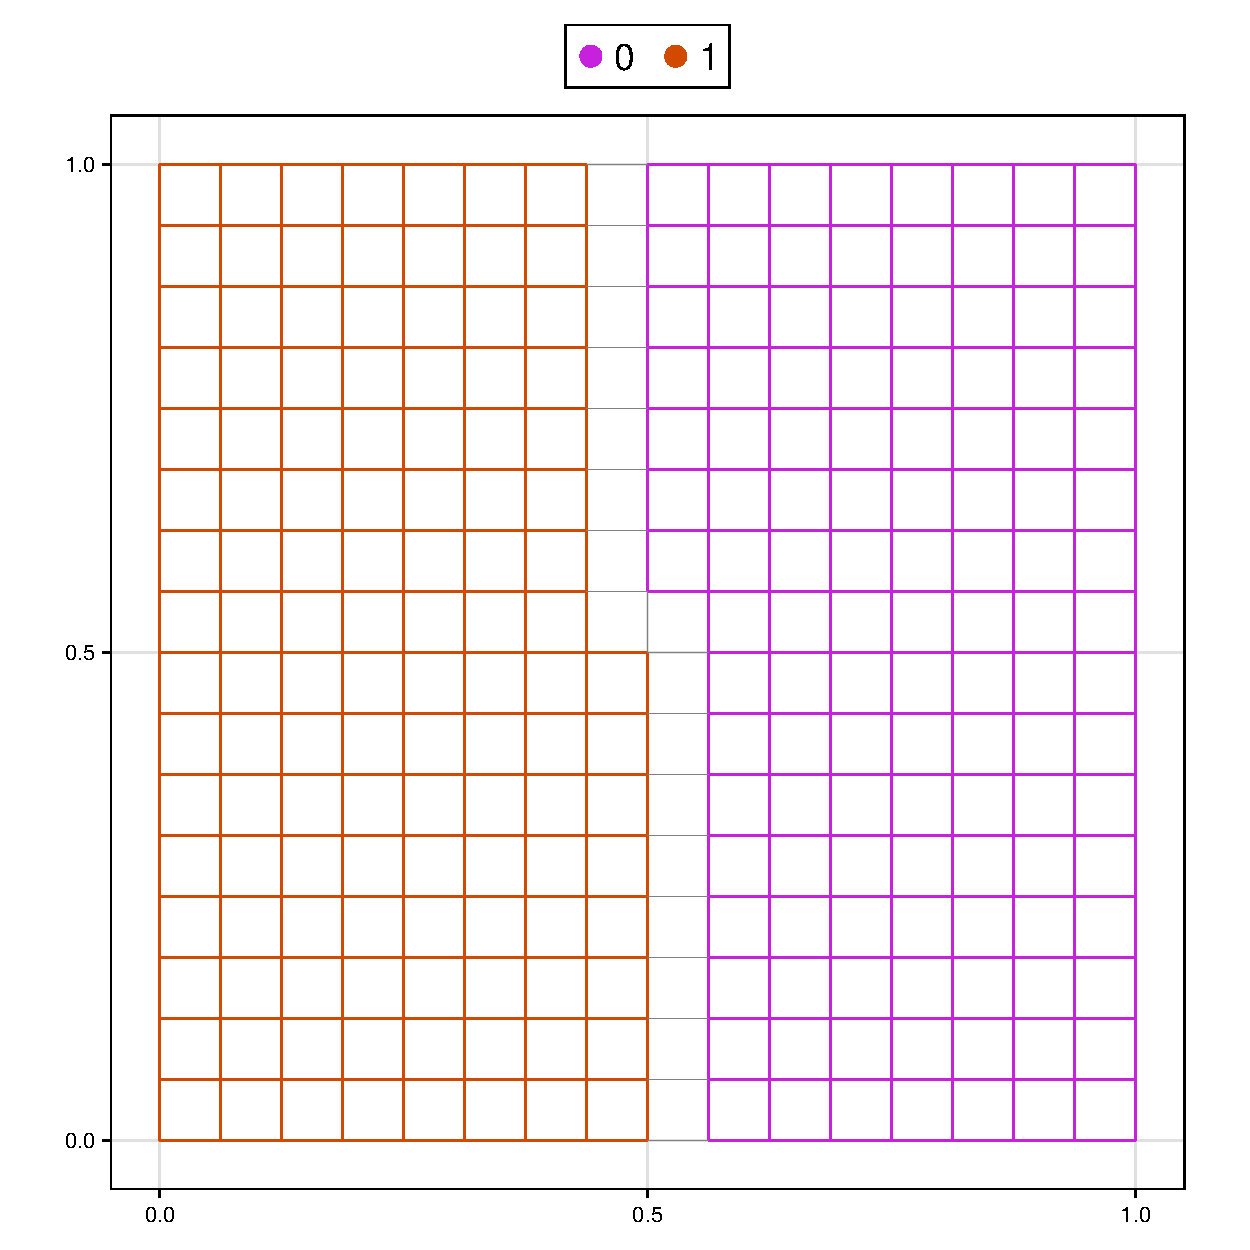
\includegraphics[width=\textwidth]{../01_graph/images/bisection/mesh3e1_metis_bisection.pdf}
    \caption{METIS}
\end{subfigure}
\caption{Bisection partitions obtained for the \texttt{mesh3e1} mesh.}
\label{fig:mesh3e1_bisections}
\end{figure}

\begin{figure}[h]
\centering
\begin{subfigure}[b]{0.24\textwidth}
    \centering
    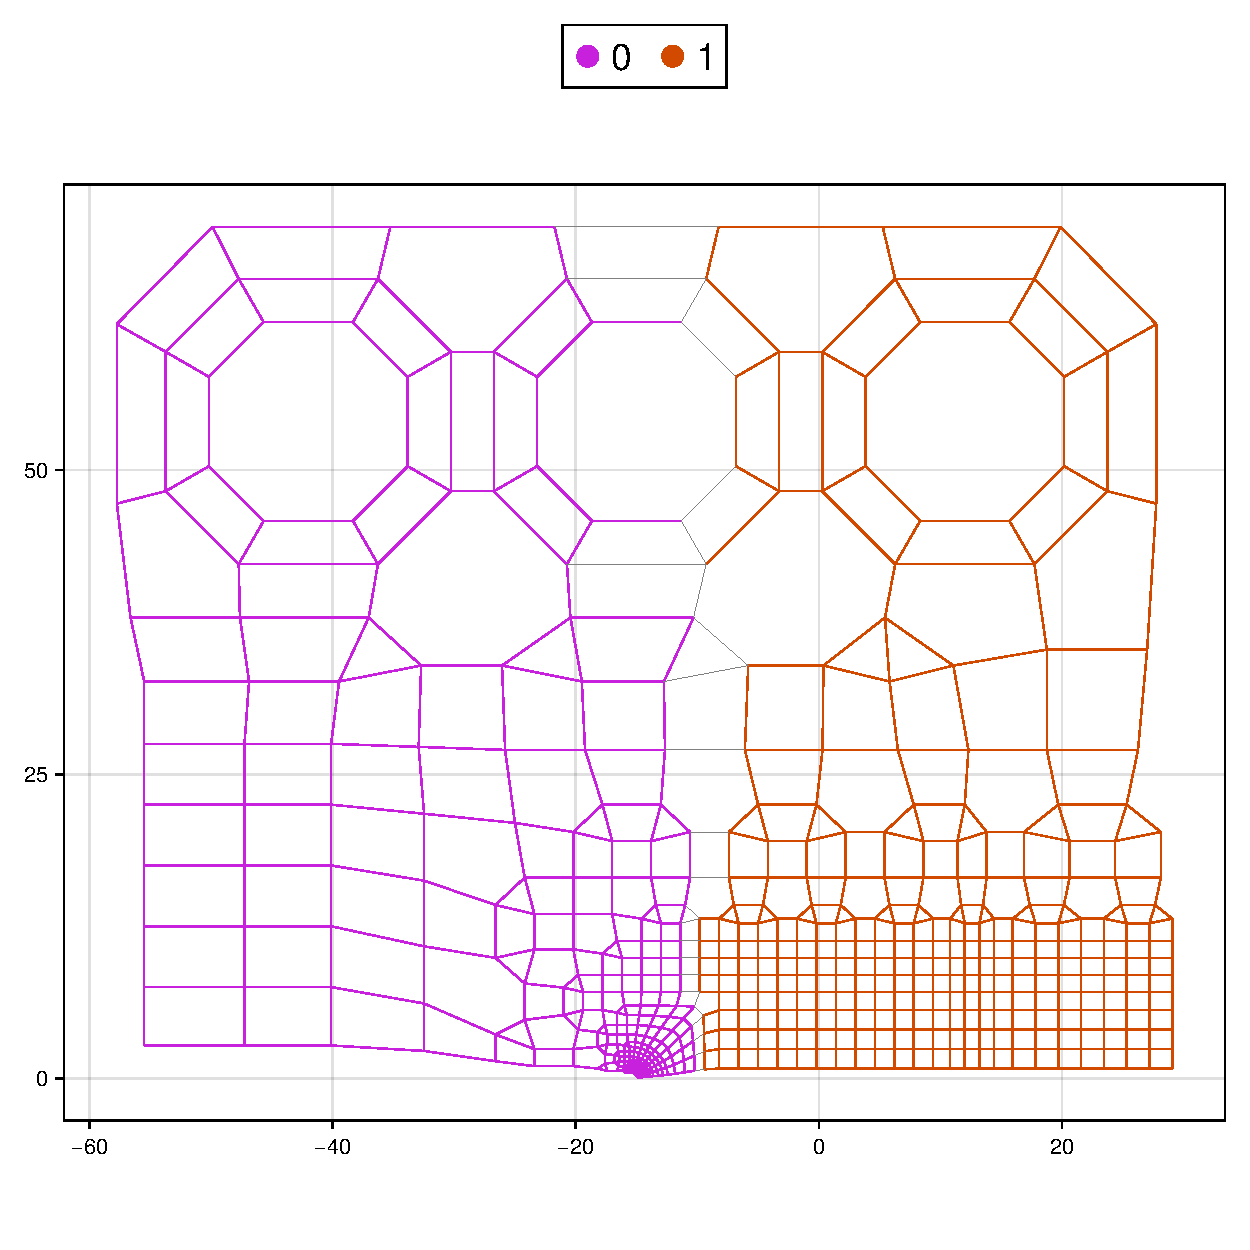
\includegraphics[width=\textwidth]{../01_graph/images/bisection/netz4504_dual_coordinate_bisection.pdf}
    \caption{Coordinate}
\end{subfigure}
\begin{subfigure}[b]{0.24\textwidth}
    \centering
    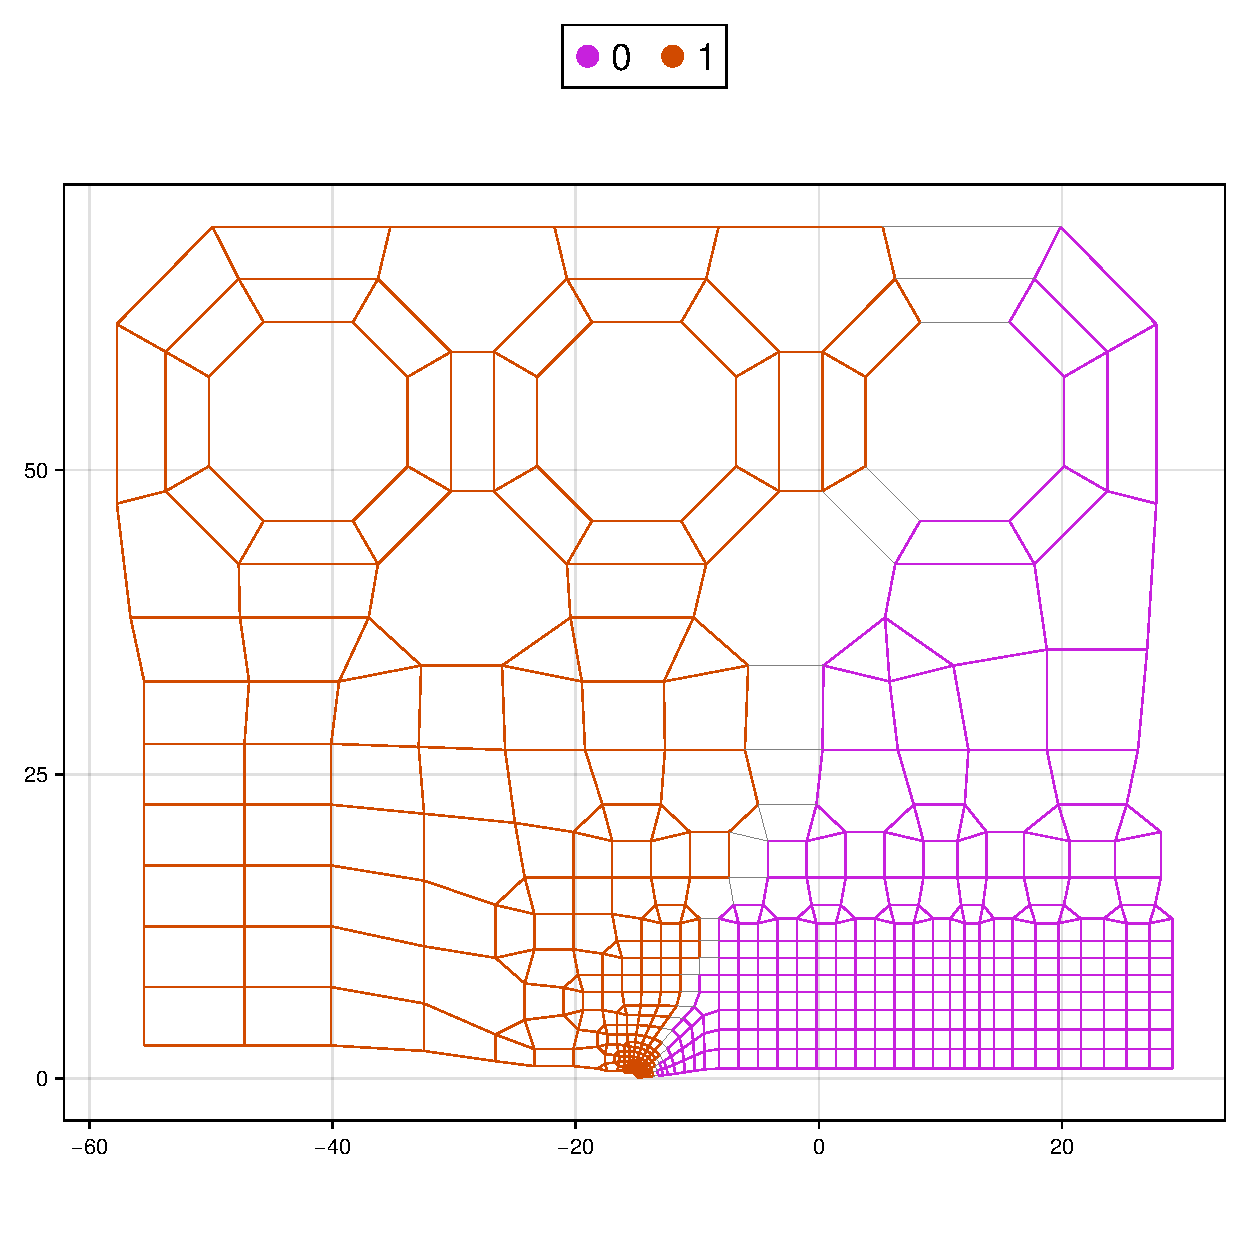
\includegraphics[width=\textwidth]{../01_graph/images/bisection/netz4504_dual_inertial_bisection.pdf}
    \caption{Inertial}
\end{subfigure}
\begin{subfigure}[b]{0.24\textwidth}
    \centering
    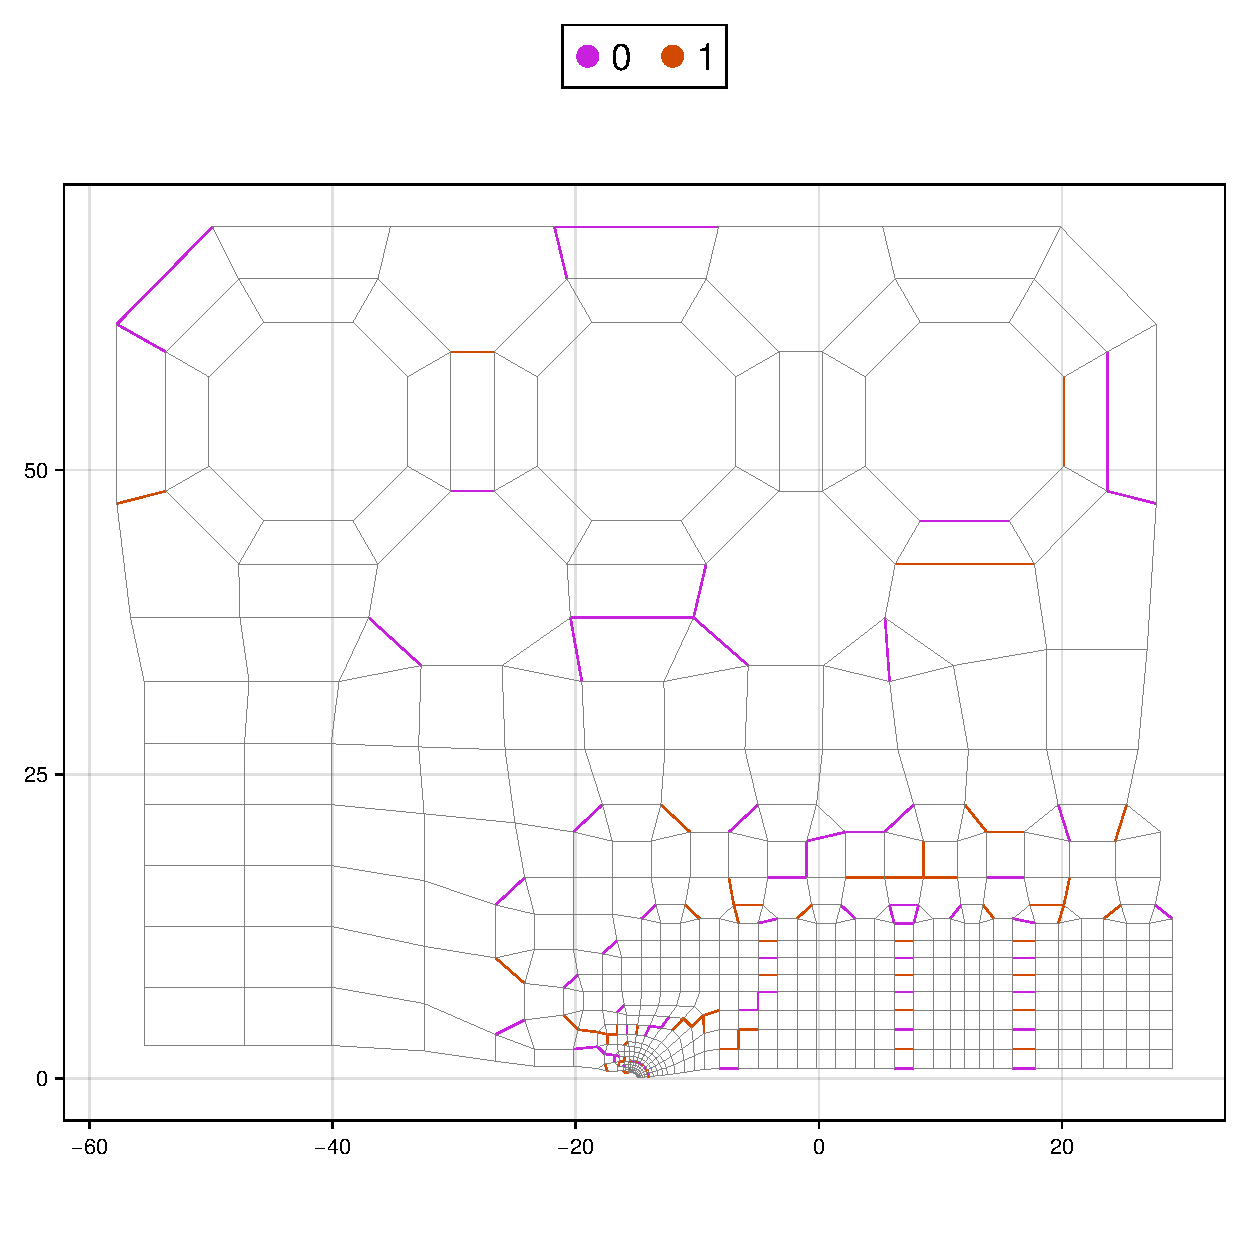
\includegraphics[width=\textwidth]{../01_graph/images/bisection/netz4504_dual_spectral_bisection.pdf}
    \caption{Spectral}
\end{subfigure}
\begin{subfigure}[b]{0.24\textwidth}
    \centering
    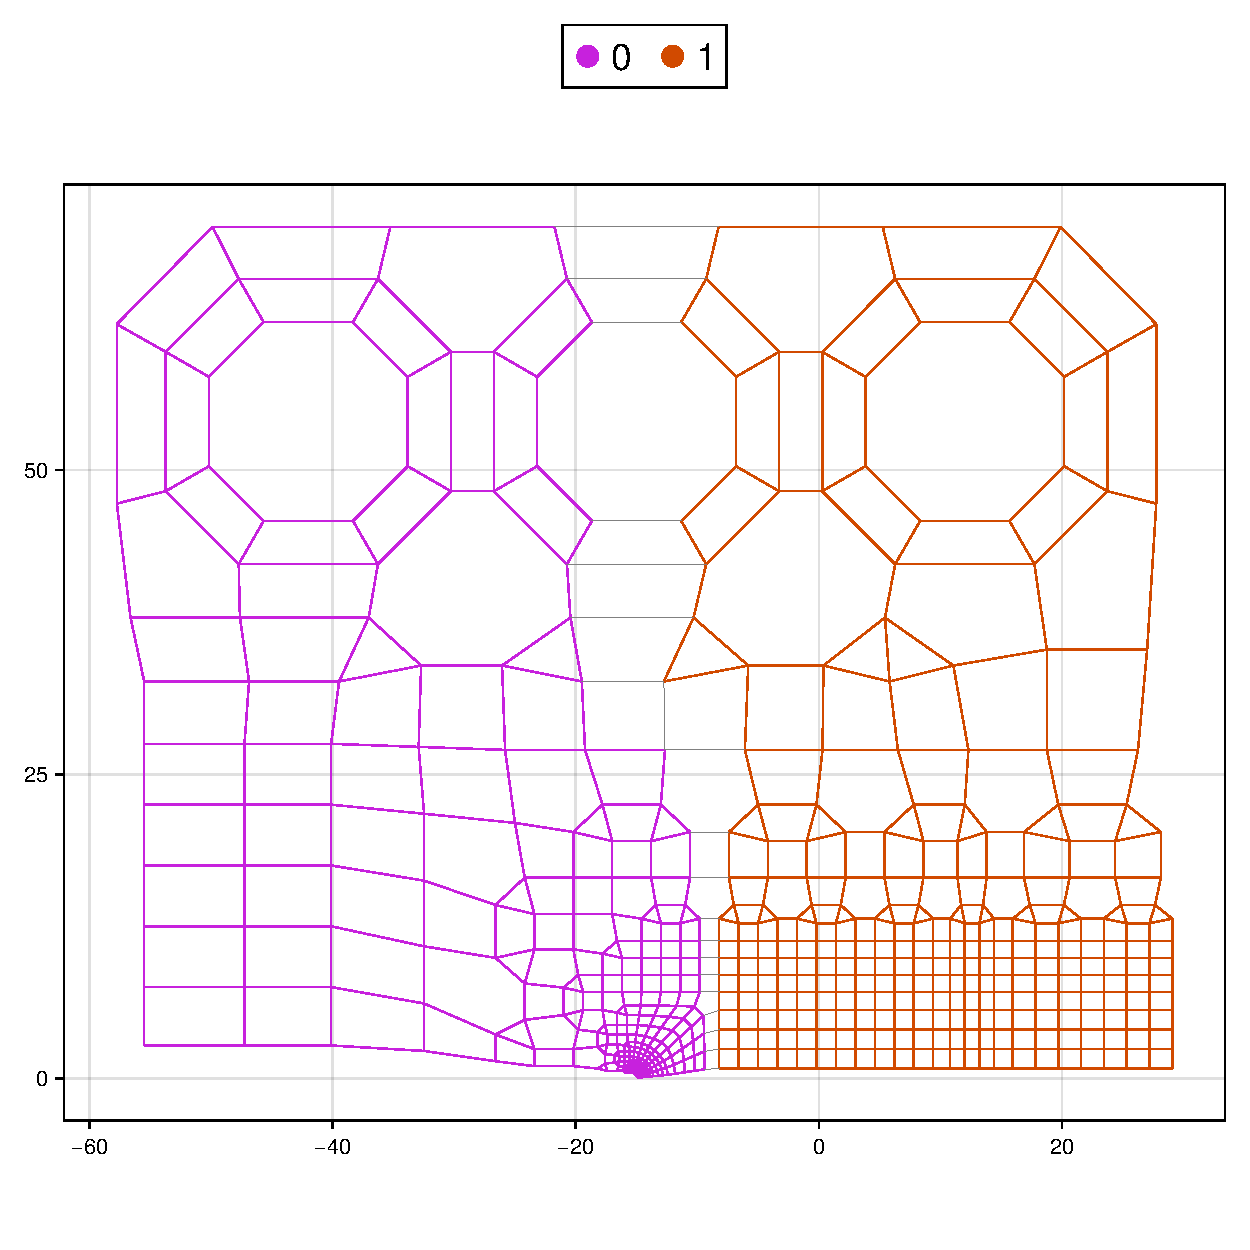
\includegraphics[width=\textwidth]{../01_graph/images/bisection/netz4504_dual_metis_bisection.pdf}
    \caption{METIS}
\end{subfigure}
\caption{Bisection partitions obtained for the \texttt{netz4504\_dual} mesh.}
\label{fig:netz4504_dual_bisections}
\end{figure}

\begin{figure}[h]
\centering
\begin{subfigure}[b]{0.24\textwidth}
    \centering
    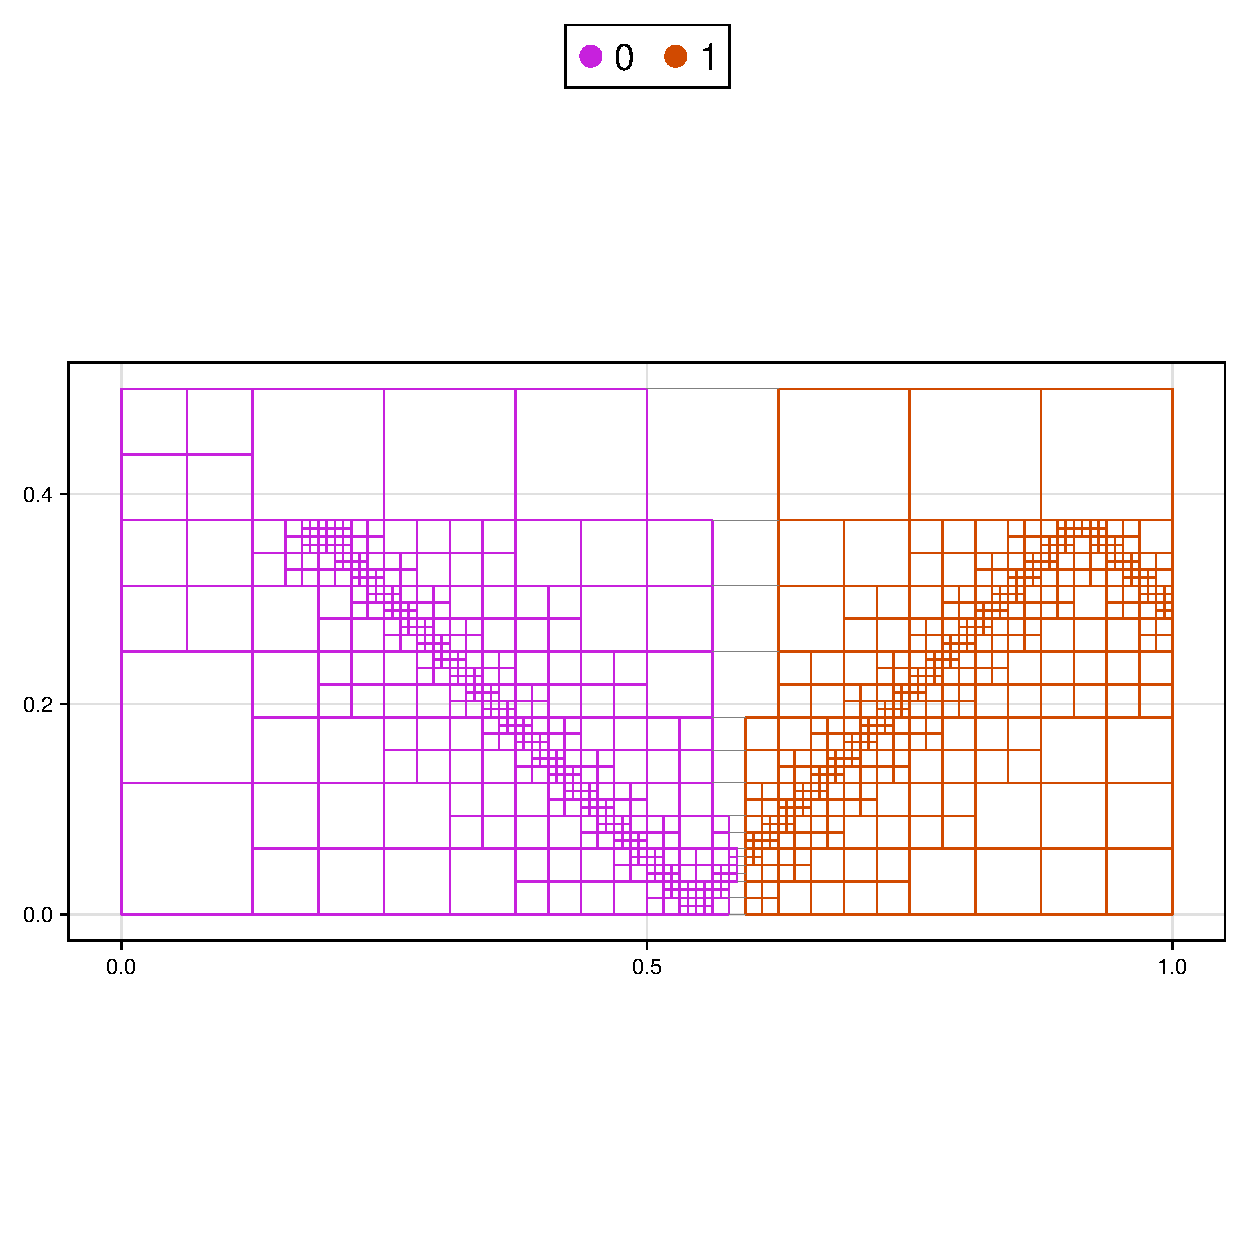
\includegraphics[width=\textwidth]{../01_graph/images/bisection/stufe_coordinate_bisection.pdf}
    \caption{Coordinate}
\end{subfigure}
\begin{subfigure}[b]{0.24\textwidth}
    \centering
    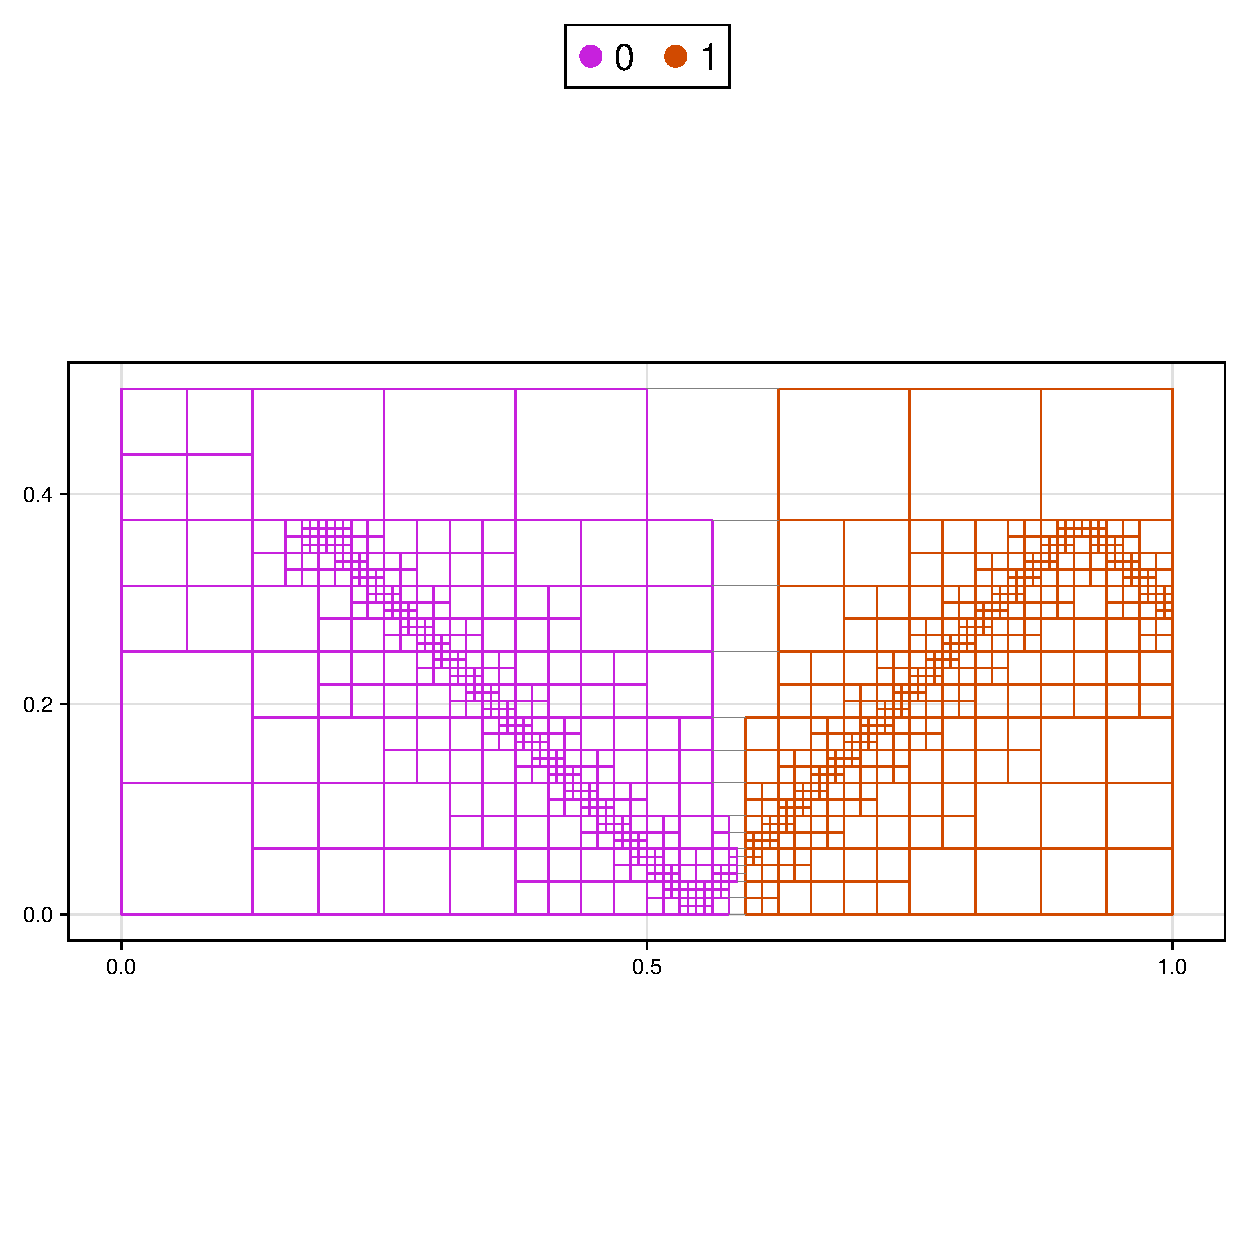
\includegraphics[width=\textwidth]{../01_graph/images/bisection/stufe_inertial_bisection.pdf}
    \caption{Inertial}
\end{subfigure}
\begin{subfigure}[b]{0.24\textwidth}
    \centering
    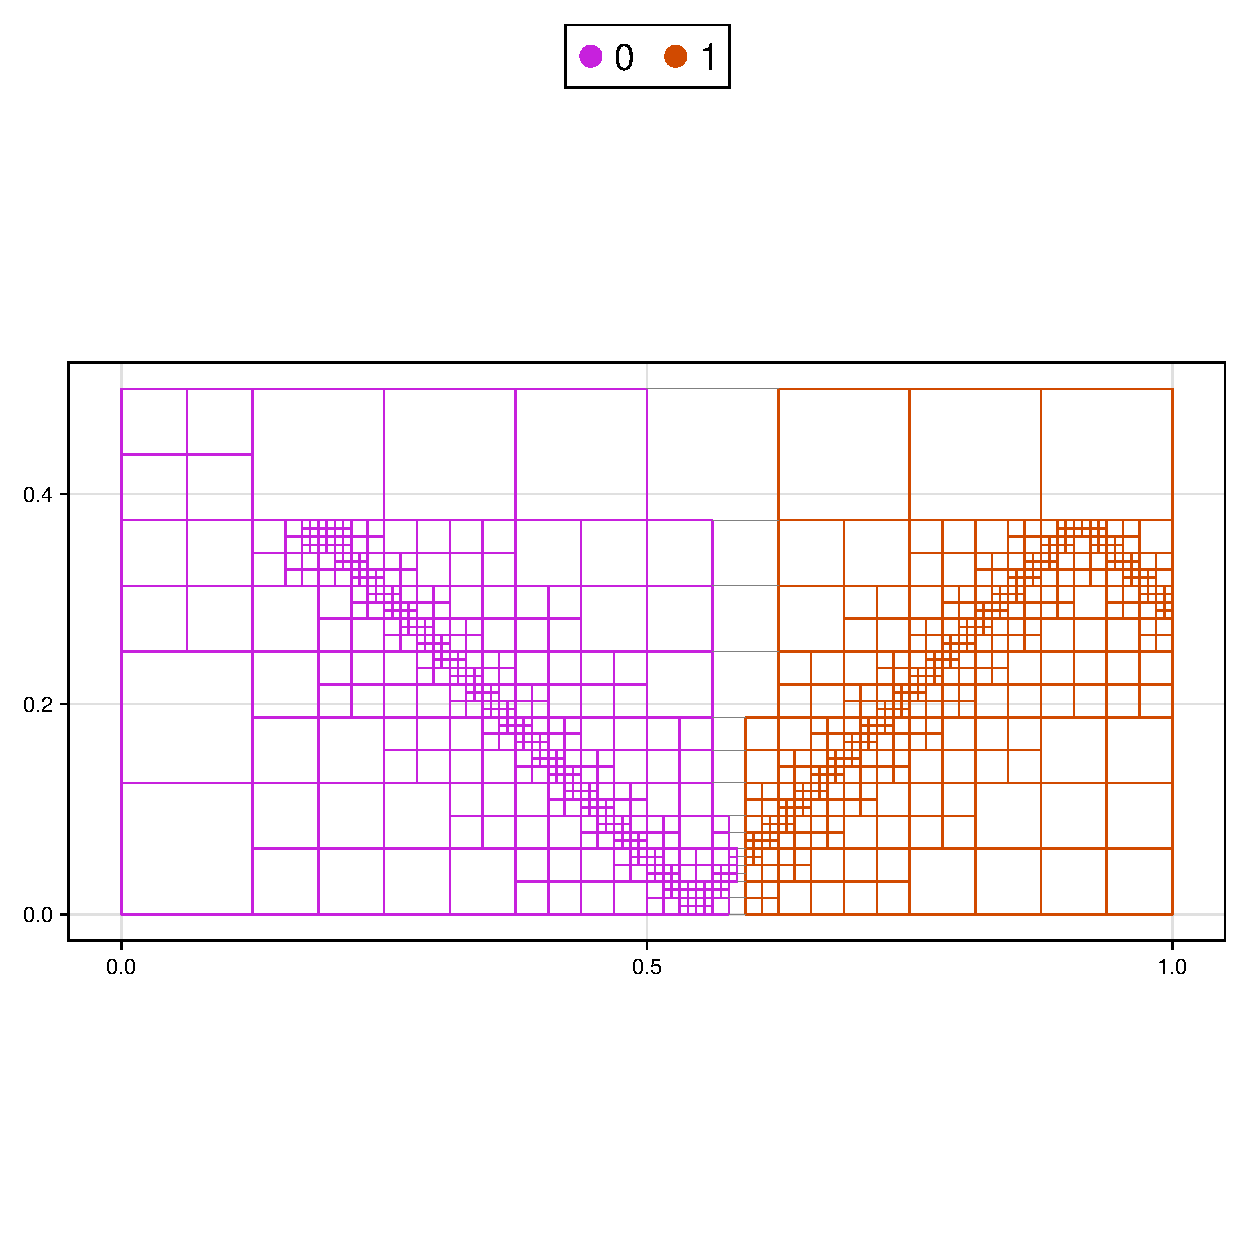
\includegraphics[width=\textwidth]{../01_graph/images/bisection/stufe_spectral_bisection.pdf}
    \caption{Spectral}
\end{subfigure}
\begin{subfigure}[b]{0.24\textwidth}
    \centering
    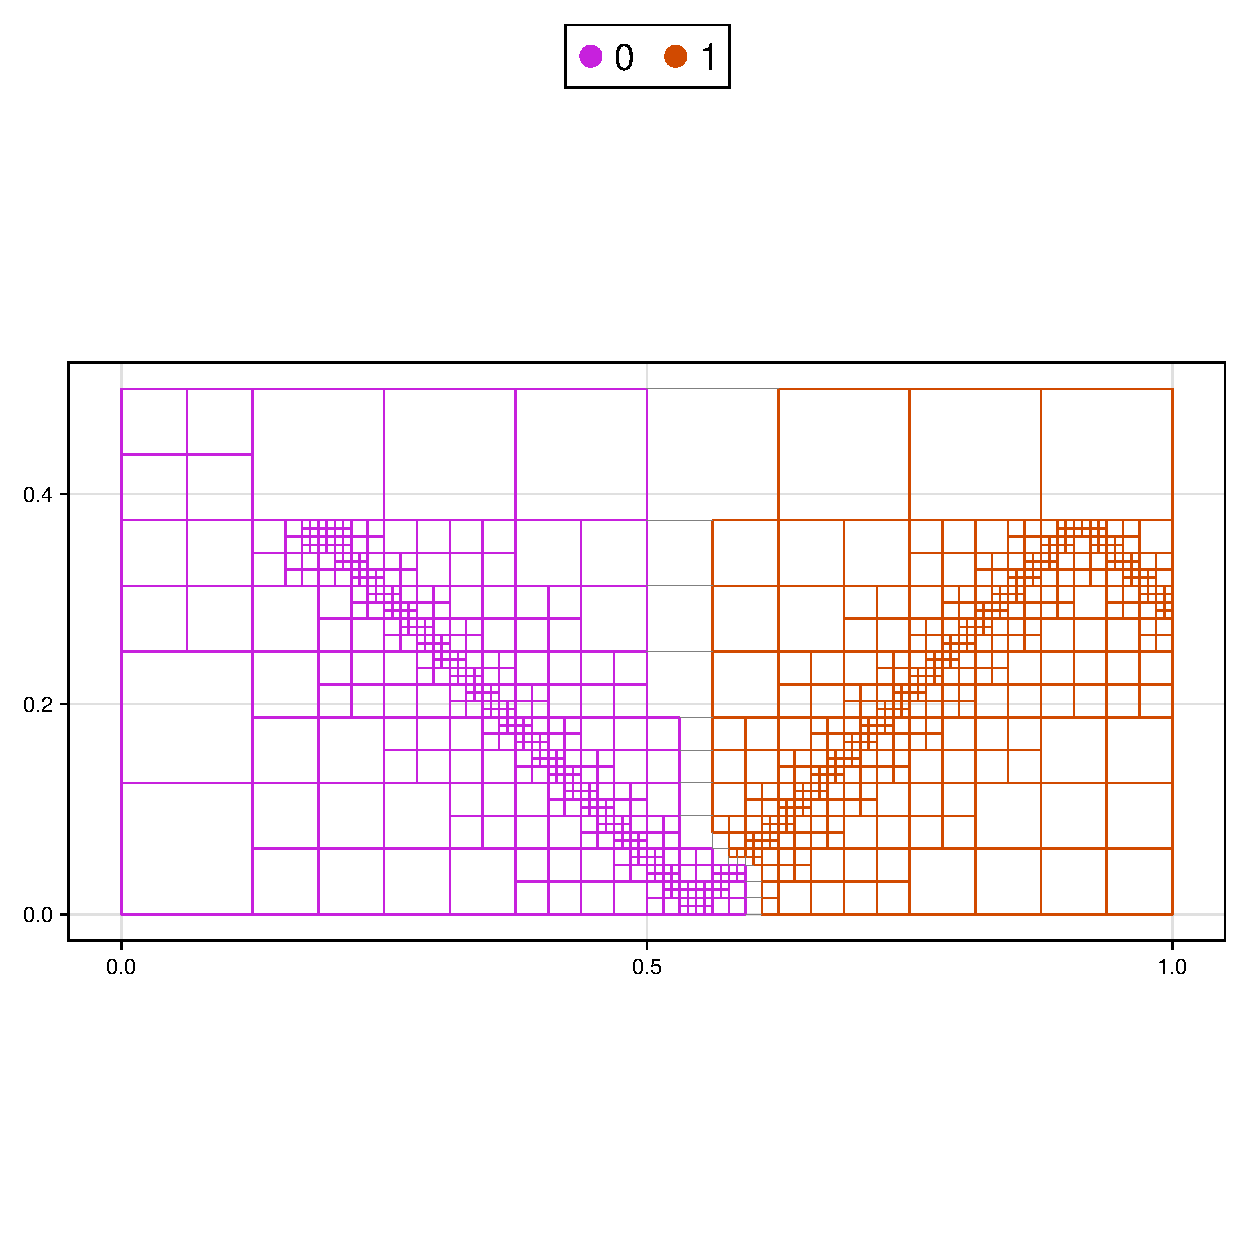
\includegraphics[width=\textwidth]{../01_graph/images/bisection/stufe_metis_bisection.pdf}
    \caption{METIS}
\end{subfigure}
\caption{Bisection partitions obtained for the \texttt{stufe} mesh.}
\label{fig:stufe_bisections}
\end{figure}

\begin{figure}[h]
\centering
\begin{subfigure}[b]{0.24\textwidth}
    \centering
    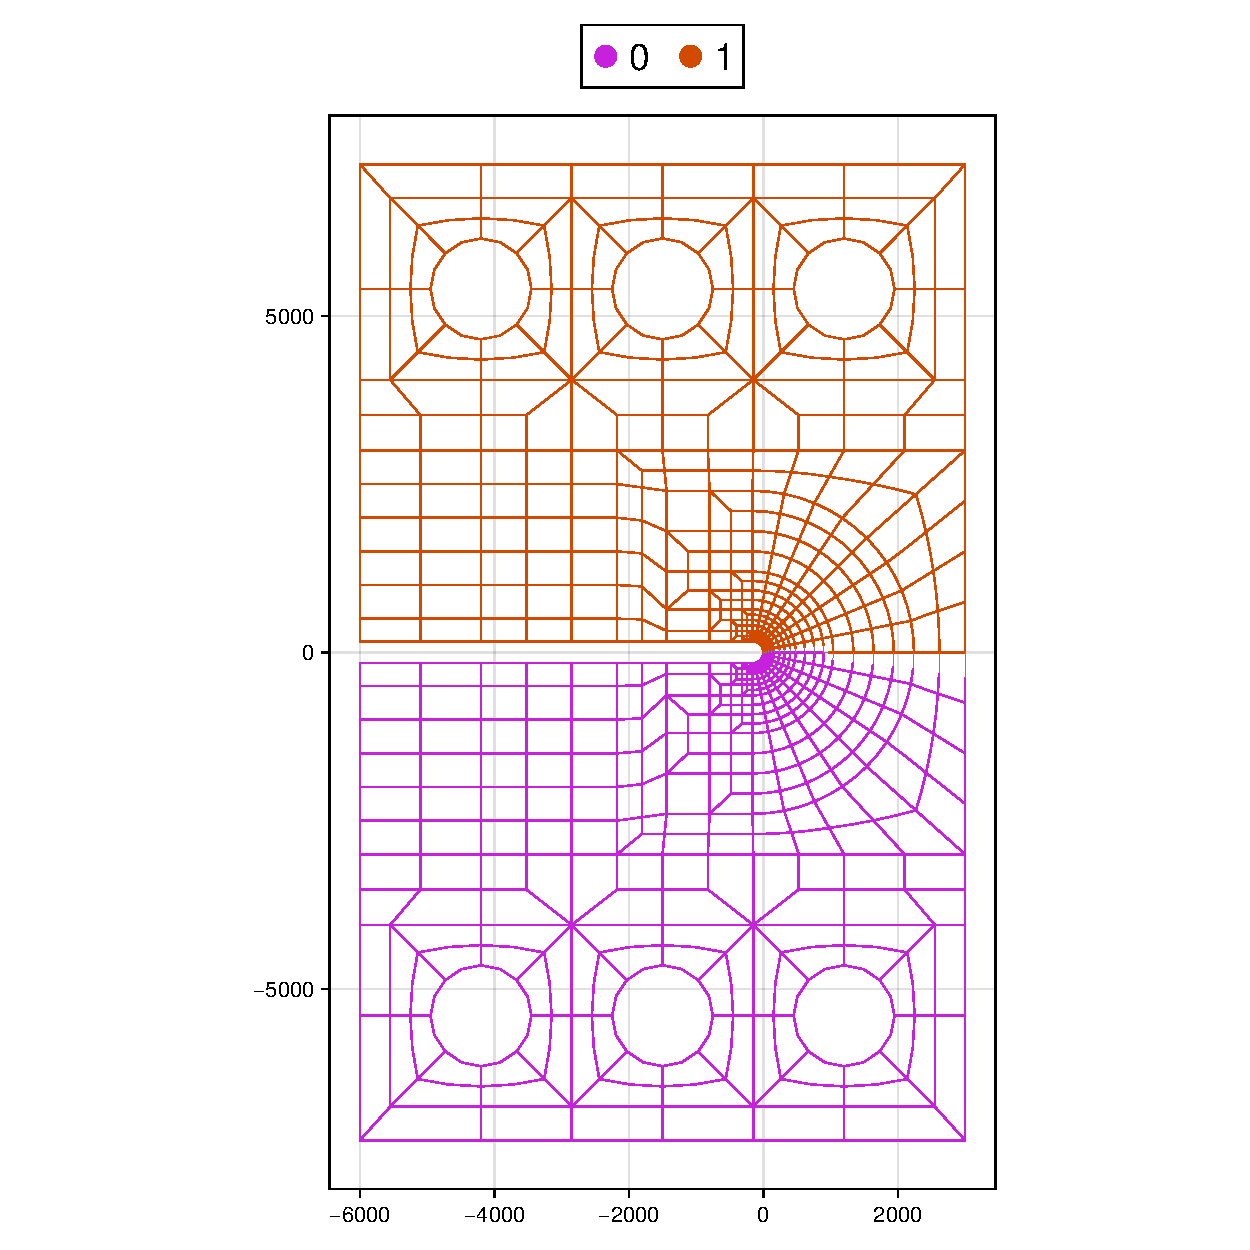
\includegraphics[width=\textwidth]{../01_graph/images/bisection/ukerbe1_coordinate_bisection.pdf}
    \caption{Coordinate}
\end{subfigure}
\begin{subfigure}[b]{0.24\textwidth}
    \centering
    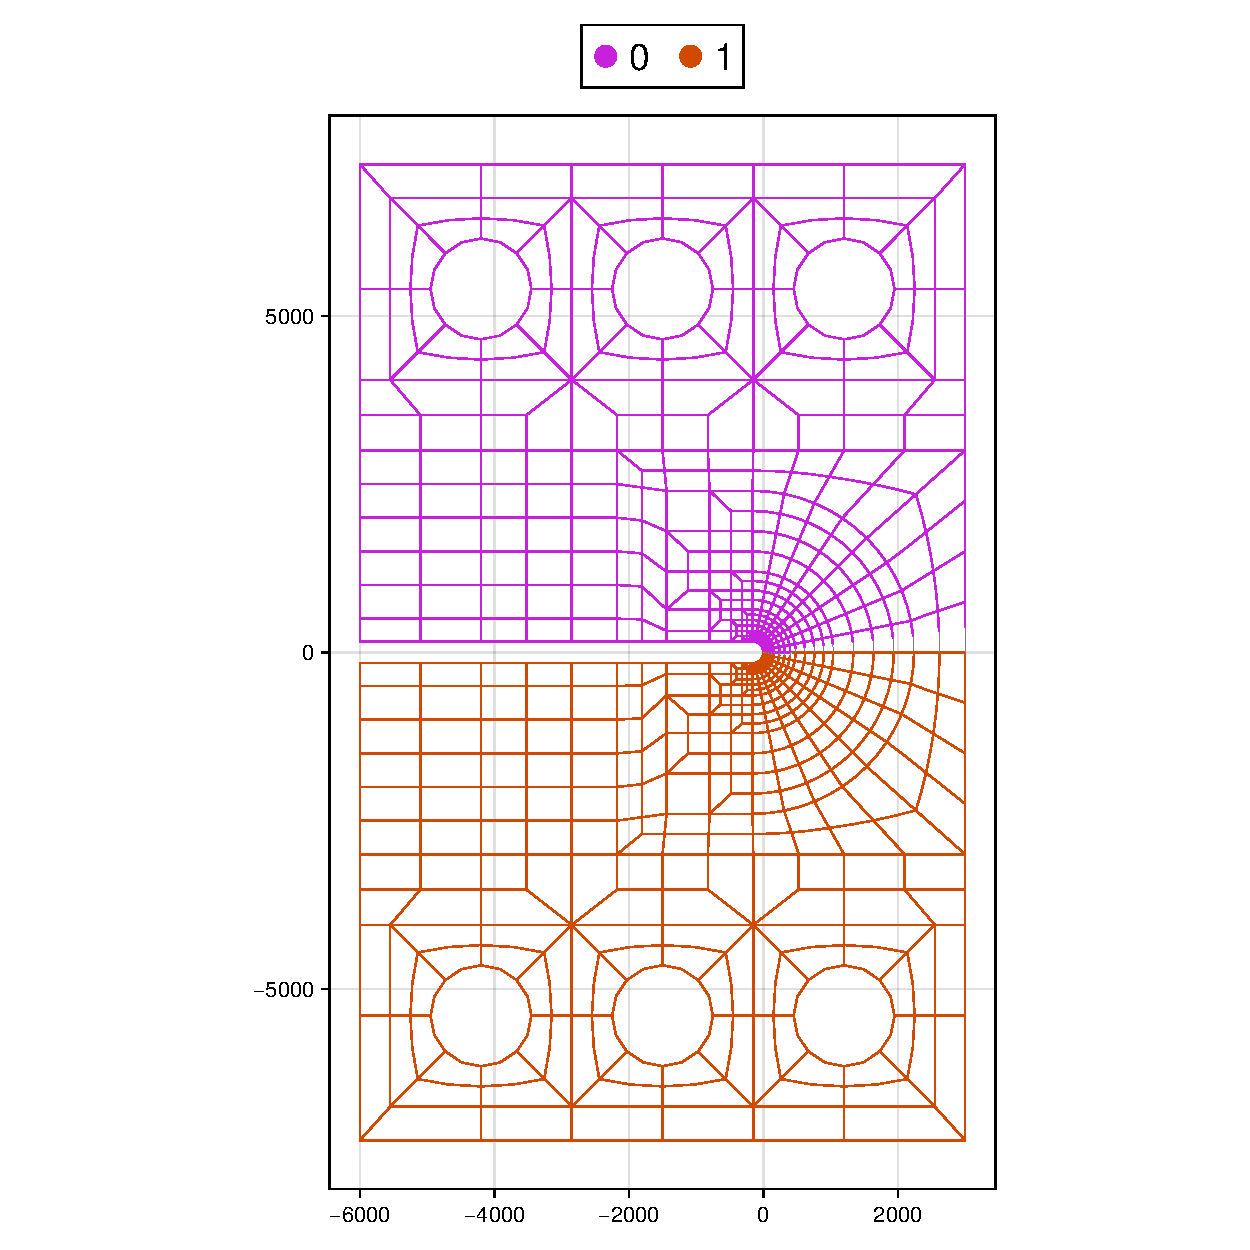
\includegraphics[width=\textwidth]{../01_graph/images/bisection/ukerbe1_inertial_bisection.pdf}
    \caption{Inertial}
\end{subfigure}
\begin{subfigure}[b]{0.24\textwidth}
    \centering
    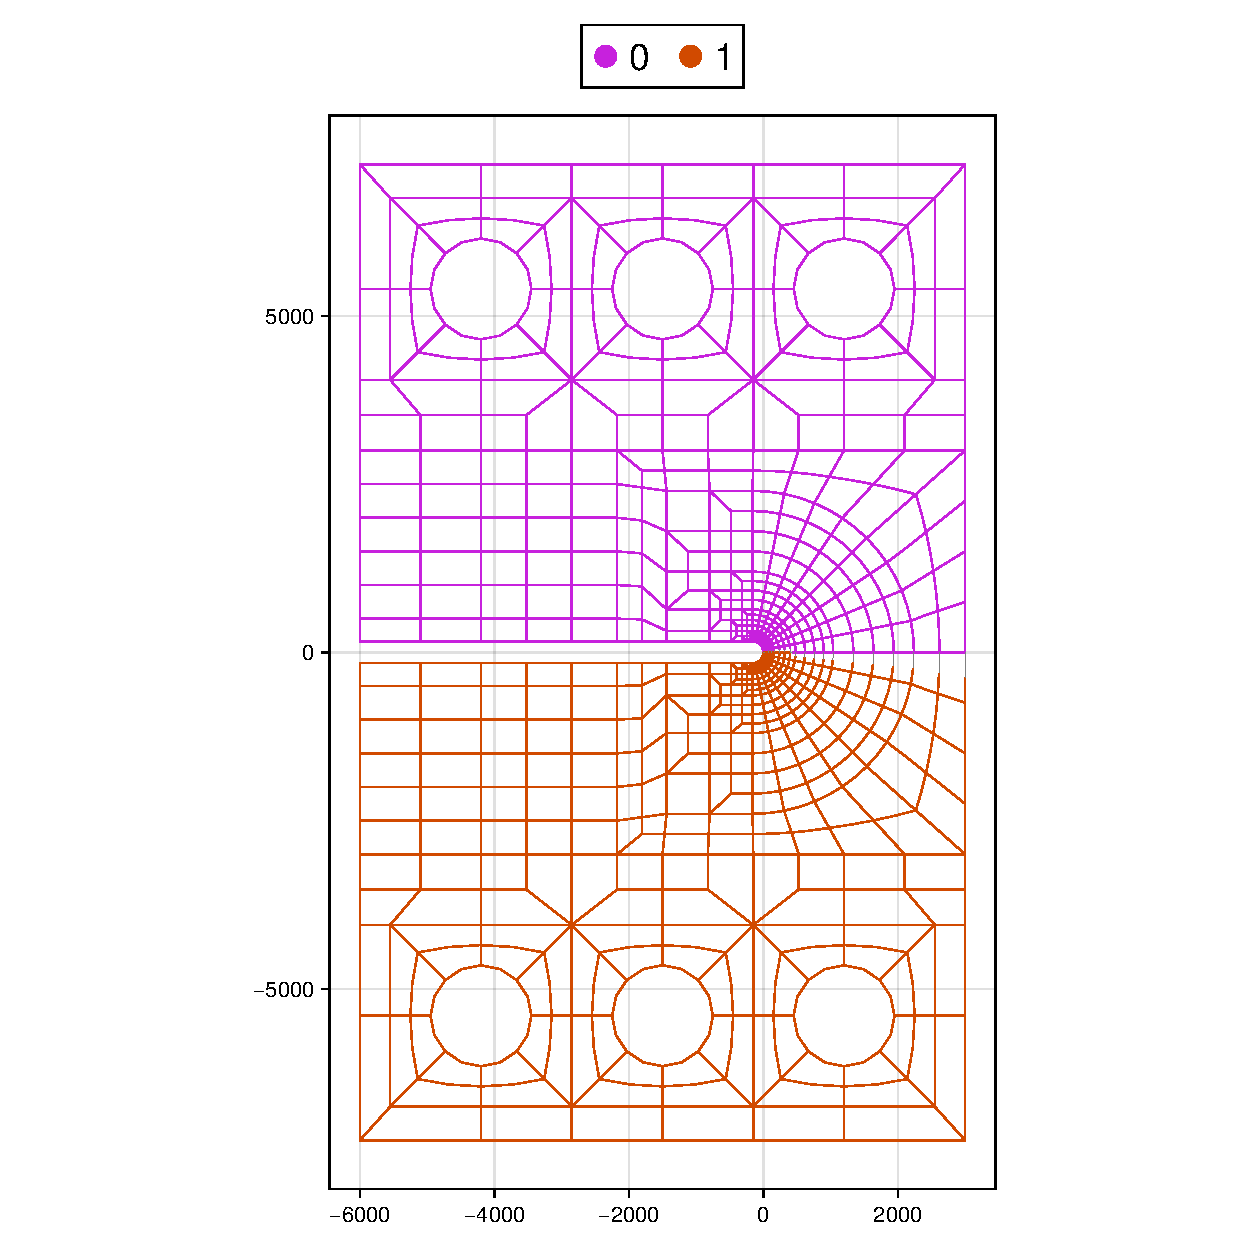
\includegraphics[width=\textwidth]{../01_graph/images/bisection/ukerbe1_spectral_bisection.pdf}
    \caption{Spectral}
\end{subfigure}
\begin{subfigure}[b]{0.24\textwidth}
    \centering
    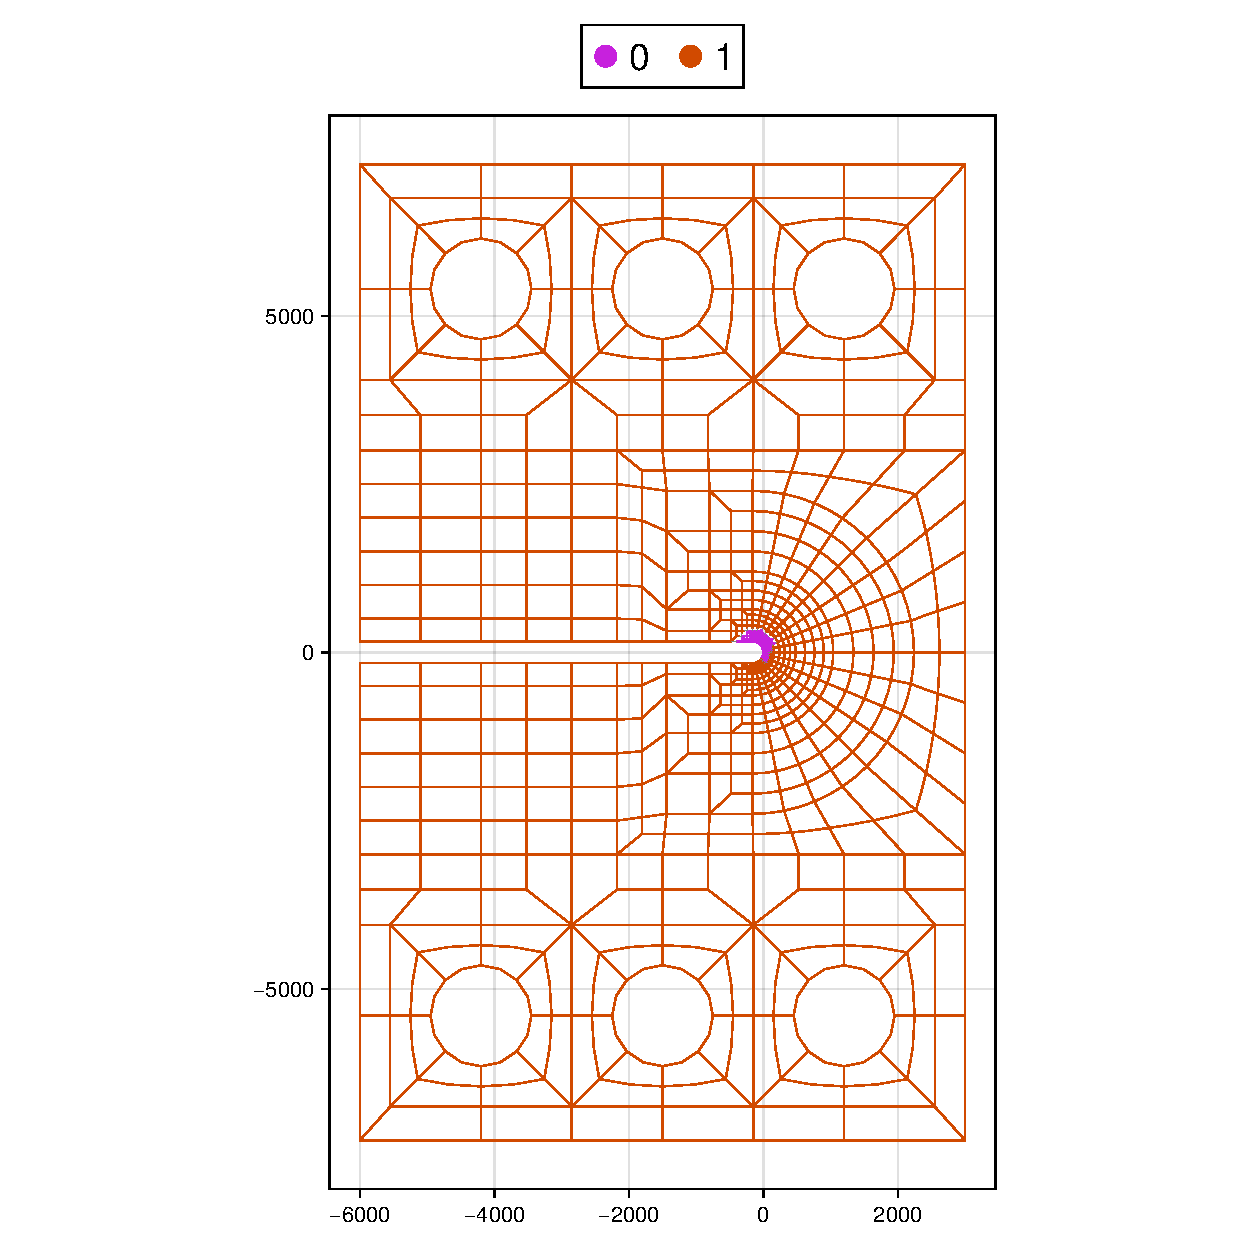
\includegraphics[width=\textwidth]{../01_graph/images/bisection/ukerbe1_metis_bisection.pdf}
    \caption{METIS}
\end{subfigure}
\caption{Bisection partitions obtained for the \texttt{ukerbe1} mesh.}
\label{fig:ukerbe1_bisections}
\end{figure}

\subsection{Recursive Bisection Algorithm}
\subsubsection{Implementation}
In lis
\newpage
\section{HPC software frameworks [50 points]}
\subsection{Mathematical Formulation}

\subsection{PETS Implementation}

\subsection{Visualization}

\subsection{Strong Scaling Analysis}


\end{document}
